\documentclass{beamer}
\includeonlyframes{current}
\setbeamertemplate{navigation symbols}{}
% \setbeamertemplate{footline}[frame number]

\title{Bayesian nonparametric model for gene expression}
\author{Eric Mittman \\ \vspace{.5cm} Advisor: Jarad Niemi}

%includes
\usepackage{amsmath, bbm, blkarray}
\usepackage{graphicx}
\usepackage{natbib}
% \usepackage{tikz}
% %include tikz
% \usepackage{tikzscale}
% \usetikzlibrary{arrows,decorations.pathmorphing,backgrounds,matrix,positioning,fit,petri, external}
\usepackage{booktabs}
\usepackage{multirow,makecell}
%\tikzexternalize[prefix=tikz/]

%theme
\usetheme{Dresden}
\usefonttheme[onlymath]{serif}
\newcommand{\frameofframes}{/}
\newcommand{\setframeofframes}[1]{\renewcommand{\frameofframes}{#1}}

\setframeofframes{of}
\makeatletter
\setbeamertemplate{footline}
  {%
    \begin{beamercolorbox}[colsep=1.5pt]{upper separation line foot}
    \end{beamercolorbox}
    \begin{beamercolorbox}[ht=2.5ex,dp=1.125ex,%
      leftskip=.3cm,rightskip=.3cm plus1fil]{author in head/foot}%
      \leavevmode{\usebeamerfont{author in head/foot}\insertshortauthor}%
      \hfill%
      {\usebeamerfont{institute in head/foot}\usebeamercolor[fg]{institute in head/foot}\insertshortinstitute}%
    \end{beamercolorbox}%
    \begin{beamercolorbox}[ht=2.5ex,dp=1.125ex,%
      leftskip=.3cm,rightskip=.3cm plus1fil]{title in head/foot}%
      {\usebeamerfont{title in head/foot}\insertshorttitle}%
      \hfill%
      {\usebeamerfont{frame number}\usebeamercolor[fg]{frame number}\insertframenumber~\frameofframes~\inserttotalframenumber}
    \end{beamercolorbox}%
    \begin{beamercolorbox}[colsep=1.5pt]{lower separation line foot}
    \end{beamercolorbox}
  }
\makeatother


%colors
% Custom colors
\usepackage{xcolor}
\definecolor{gold}{HTML}{F1BE48}
\definecolor{red}{HTML}{C8102E}
\setbeamercolor{upcol}{fg=black,bg=red}
\setbeamercolor{lowcol}{fg=black,bg=gold!40}
\usecolortheme[named=red]{structure}

%macros
\newcommand{\mc}{\mathcal}
\newcommand{\mb}{\mathbb}
\newcommand{\op}{\operatorname}
\newcommand{\ind}{\stackrel{ind}{\sim}}
\newcommand{\iid}{\stackrel{ind}{\sim}}

\AtBeginSection[]{
  \begin{frame}
  \vfill
  \centering
  \begin{beamercolorbox}[sep=8pt,center,shadow=true,rounded=true]{title}
  \usebeamerfont{title}\secname\par%
  \end{beamercolorbox}
  \vfill
  \end{frame}
}

\graphicspath{{../chapter1/figures_tables/}{../chapter2/figures_tables/}{../chapter3/figures_tables/}}

\begin{document}


\frame{\titlepage}

% \begin{frame}
% \frametitle{Table of Contents}
% \tableofcontents
% \end{frame}

%%% Section 0: Data problem
\section[GE/RNA-seq]{Gene expression and RNA-seq}

\begin{frame}%%[label=current]
  \frametitle{``Gene expression" $=$ Transcript abundance}
  {\scriptsize \citep[\textit{Statistical Analysis of Next Generation Sequencing Data}]{datta2014}}
  The Central Dogma of Biology says:
  \begin{itemize}
    \pause\item DNA encodes all biological information
    \pause\item Genes (regions of the DNA) encode directions for assembling proteins
    \pause\item messenger RNA (mRNA) conveys ``transcripts" of these directions to the ribosomes where they are assembled 
  \end{itemize}
  \pause Transcript abundance is proxy for gene expression.
\end{frame}

\begin{frame}%%[label=current]
\frametitle{Gene expression profiling - RNA-seq}
  \pause RNA-seq is:
  \vspace{.5cm}
  \begin{itemize}
    \pause \item "whole transcriptome shotgun sequencing"
    \pause \item simultaneously measurement of transcript abundance of thousands of genes
    \pause \item sequencing is high resolution
  \end{itemize}
  
  \vspace{.5cm}
  Stages of RNA-seq data production:
  \vspace{.5cm}
  \begin{itemize}
    \pause \item isolate mRNA
    \pause \item fragmentation
    \pause \item amplification
    \pause \item sequencing/matching fragments back to genes/features (counts)
  \end{itemize}
\end{frame}



\begin{frame}%[label=current]
  \frametitle{Using gene expression to identify heterosis}
  \begin{columns}
    \begin{column}{.3\textwidth}
      \begin{table}
        \begin{tabular}{c}
          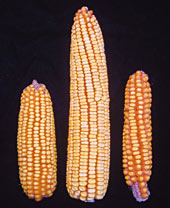
\includegraphics[height=.35\textheight]{BFMears}\\
          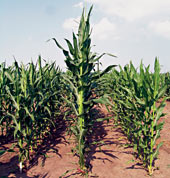
\includegraphics[height=.35\textheight]{BFMfield}
        \end{tabular}
        {\scriptsize \url{https://archive.news.iastate.edu/news/2006/may/vigor.shtml}}
      \end{table}
    \end{column}
    
    \begin{column}{.7\textwidth}
    \centering
    \scalebox{.9}{
      \begin{beamerboxesrounded}[upper=upcol,lower=lowcol,shadow=true]{Heterosis}
        \begin{itemize}
          \pause\item Heterosis $=$ ``Hybrid vigor"
          \pause \item Superior traits in hybrid offpring compared with inbred parents
          \pause \item Want to identify genetic links
        \end{itemize}
        \vspace{.5cm}
        \pause average hybrid expression more extreme than parental expression
        \begin{itemize}
          \pause \item high-parent heterosis (HPH):\\low parent $<$ high parent $<$ hybrid
          \pause \item low-parent heterosis (LPH):\\ hybrid $<$ low parent $<$ high parent
        \end{itemize}
      \end{beamerboxesrounded}
      \onslide<1->
    }
    \end{column}
  \end{columns}
\end{frame}

\begin{frame}%[label=current]
  \frametitle{Identifying heterosis: statistical approach}
  Problem statement: identify genes for which either
  {\small
  \begin{enumerate}
    \pause \item $H_{HPH,g}: (\mbox{hybrid mean expression} > \mbox{high-parent mean expression)}$\\ is likely \pause or
    \item $H_{LPH,g}: (\mbox{hybrid mean expression} < \mbox{low-parent mean expression)}$\\ is likely.
  \end{enumerate}
  }
  
  \begin{itemize}
    \pause \item Null hypothesis testing is problematic; p-values not uniform under null, so methods for multiple correction do not apply
    \pause \item Bayesian methods allow direct estimation of, e.g., $Pr(H_{HPH,g} \mbox{ is true})$
    \pause \item Hierarchical model to borrow information across genes
  \end{itemize}
\end{frame}

\section{Data}
\begin{frame}%%[label=current]
  \frametitle{Data from \citet{paschold}}
  Produced 16 RNA samples from primary roots of 3.5 day old maize seedlings (each produced from 10 individuals) with aim to identify genes responsible for hybrid vigor (heterosis).
  \vspace{.5cm}
  \pause\begin{beamerboxesrounded}[upper=upcol,lower=lowcol,shadow=true]{}
  \begin{itemize}
    \item 2 inbred lines (homozygous): B73, Mo17
    \item 2 reciprocal hybrid crosses: B73$\times$Mo17, Mo17$\times$B73
    \item 4 replicates of each variety
    \item sequencing done on 2 flow cells, genotypes balanced across flow cells
  \end{itemize}
  \end{beamerboxesrounded}
\end{frame}

\begin{frame}%[label=current]
  \frametitle{RNA-seq data}
  \begin{columns}
    \column{\dimexpr\paperwidth-10pt}
    % latex table generated in R 3.4.2 by xtable 1.8-2 package
    % Fri Dec 01 15:02:44 2017
    \begin{table}[ht]
      \scalebox{.6}{
        \setlength\tabcolsep{1.5pt} % default value: 6pt
        \begin{tabular}{c|l|rrrr|rrrr|rrrr|rrrr}
          \toprule
          GeneID & \multicolumn{1}{c}{ex. of} &  \multicolumn{4}{c}{B73} & \multicolumn{4}{c}{B73xMo17} & \multicolumn{4}{c}{Mo17xB73}& \multicolumn{4}{c}{Mo17}  \\
          \midrule
          GRMZM2G306345 & HPH & 1431 & 1199 & 1235 & 1569 & 2055 & 1652 & 2149 & 2168 & 2415 & 1815 & 2142 & 2369 & 1127 & 987 & 1672 & 1518 \\
          GRMZM2G149543 &  LPH &  86 &  62 & 131 & 128 &  52 &  43 &  85 &  95 &  60 &  23 &  63 &  74 &  85 &  71 & 178 & 205 \\
          GRMZM2G079613 &  mixed & 122 &  98 & 146 & 150 &  73 &  77 & 159 & 127 & 178 & 122 & 259 & 252 & 108 & 103 & 207 & 171 \\
          AC194005.3\_FG004 &  neither &  30 &  31 &  42 &  48 &  17 &  15 &  22 &  26 &  16 &  13 &  16 &  22 &   2 &   2 &   2 &   2 \\ 
          \vdots & & & & & & & & & & & & & & & & &\\ \midrule
          Raw total && 1.2E7 & 1.0E7  & 0.9E7  & 1.0E7 & 1.1E7 & 1.0E7 &1.0E7  &1.0E7 &1.1E7 &1.0E7 &1.0E7  &1.0E7 &1.0E7  &0.9E7 &1.0E7  &1.0E7\\
          \bottomrule
        \end{tabular}
      }
    \end{table}
    \begin{itemize}
      \pause \item Counts (contain zeros)
      \pause \item Small samples are typical
      \pause \item Tens of thousands of genes
    \end{itemize}
  \end{columns}
\end{frame}

%%%%%%%%%%%%%
\section[Model Intro]{Modeling RNA-seq data}

\begin{frame}
  \frametitle{Log-linear modeling of RNA-seq data}
  Approach of \citep{voom}:
  \begin{itemize}
    \item Linear model for log counts per million (log-cpm)
    \item Nonparametric correction for mean-variance trend (precision weights, $w_{gn}$)
    \item $r_{gn} = \mbox{count for gene }g \mbox{, sample }n;\quad g=1,\ldots,G,\quad n=1,\ldots,N$
    \item $R_n = \mbox{library size for sample }n$
    \item $y_{gn} = \log_2 \left(\frac{r_{gn}+0.5}{R_n+1}\times 10^6\right)$
    \item Model: $y_{gn} = x_n\beta_g + \epsilon_{gn};\; \epsilon_{gn} \ind \op{N}(0,\sigma^2_g/w_{gn})$
  \end{itemize}
\end{frame}

\begin{frame}%%[label=current]
  \frametitle{Gene-specific parameters}
  \begin{beamerboxesrounded}[upper=upcol,lower=lowcol,shadow=true]{model matrix} 
    \centering
    \scalebox{.6}{
      \begin{equation*} X=
        \begin{blockarray}{rrrrrr}
          \mbox{Sample} & \mbox{intercept} & \mbox{parental HD} & \mbox{hybrid} & \mbox{hybrid HD} & \mbox{flow cell}\\
          \begin{block}{r(rrrrr)}
            \mbox{B73}_1  & 1 &  1 & 0 & 0 & 0\\
            \mbox{B73}_2  & 1 &  1 & 0 & 0 & 0\\
            \mbox{B73}_3  & 1 &  1 & 0 & 0 & 1\\
            \mbox{B73}_4  & 1 &  1 & 0 & 0 & 1\\
            \mbox{B73}\times\mbox{Mo17}_1  & 1 &  0 & 1 & 1 & 0\\
            \mbox{B73}\times\mbox{Mo17}_2  & 1 &  0 & 1 & 1 & 0\\
            \mbox{B73}\times\mbox{Mo17}_3  & 1 &  0 & 1 & 1 & 1\\
            \mbox{B73}\times\mbox{Mo17}_4  & 1 &  0 & 1 & 1 & 1\\
            \mbox{Mo17}\times\mbox{B73}_1  & 1 &  0 & 1 & -1 & 0\\
            \mbox{Mo17}\times\mbox{B73}_2  & 1 &  0 & 1 & -1 & 0\\
            \mbox{Mo17}\times\mbox{B73}_3  & 1 &  0 & 1 & -1 & 1\\
            \mbox{Mo17}\times\mbox{B73}_4  & 1 &  0 & 1 & -1 & 1\\
            \mbox{Mo17}_1 & 1 & -1 & 0 & 0 & 0\\
            \mbox{Mo17}_2 & 1 & -1 & 0 & 0 & 0\\
            \mbox{Mo17}_3 & 1 & -1 & 0 & 0 & 1\\
            \mbox{Mo17}_4 & 1 & -1 & 0 & 0 & 1
          \end{block}
        \end{blockarray}
      \end{equation*}
    }
  \end{beamerboxesrounded}
\end{frame}

\begin{frame}%%[label=current]
  \frametitle{Gene-specific parameter estimates}
  {\centering
    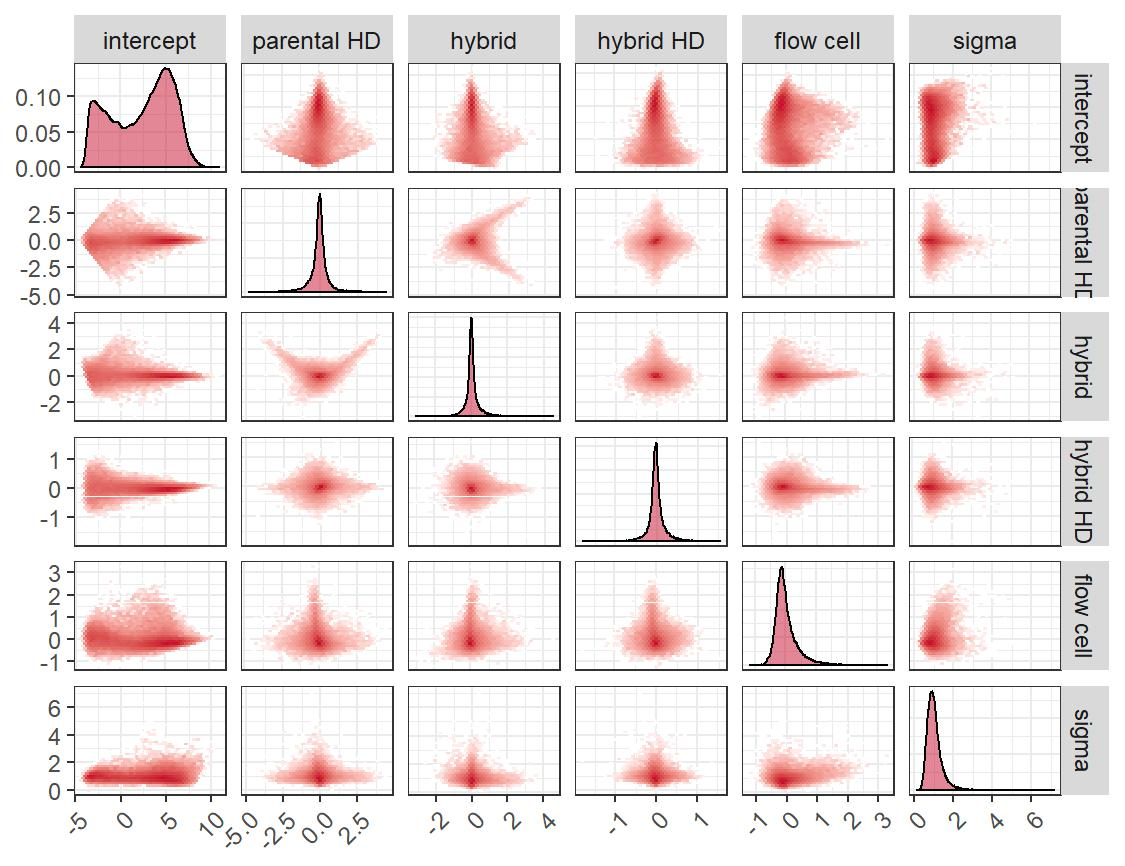
\includegraphics[width=.8\textwidth]{pairs1}\\
  }
\end{frame}
  
\begin{frame}%[label=current]
  \frametitle{Rationale for BNP}
  Idea: $\beta_g \ind \mathcal{P},\quad \mathcal{P} ~ F$
  
  Argument for Bayesian non-parametric (BNP) model:
  \begin{itemize}
    \item Hierarchical model to borrow information
    \item Avoid unrealistic model assumptions
    \item General solution; not case specific
  \end{itemize}
\end{frame}

%%%%%%%%%%%%%%
\section[DP intro]{The Dirichlet process}

\begin{frame}%%[label=current]
  \centering
  \scalebox{.8}{
    \begin{beamerboxesrounded}[upper=upcol,lower=lowcol,shadow=true]{Stick-breaking representation}
      $\mathcal{P}$ = a random probability measure$\\
      \pause $\mathcal{P} \sim \op{DP}(\alpha Q) \implies$
      \begin{itemize}
        \pause \item $\mathcal{P} \stackrel{d}{=} \sum_{k=1}^\infty \pi_k \delta_{\tilde{\mu}_k},\;$ where $\delta_{\cdot}$ is the Dirac delta function, \pause
        \item $\tilde{\mu}_k \ind Q$ \pause and
        \item $\frac{\pi_k}{1-\sum_{\ell<k} \pi_\ell}=\nu_k \ind \op{Be}(1,\alpha)$
      \end{itemize}
      
      \vspace{.5cm}
      
      \pause Finite approximation: choose large $K$, set $\nu_K=1$, implying, for $\ell>K$, $\pi_\ell=0$.\\
      \onslide<1->
      \citep{sethuraman,ishwaran2000}
    \end{beamerboxesrounded}
  }
\end{frame}

\begin{frame}%%[label=current]
  \frametitle{DP as infinite mixture ($Q=\op{N}(0,1)$)}
  \scalebox{.7}{
    \begin{table}
      \centering
      \begin{tabular}{crl}
        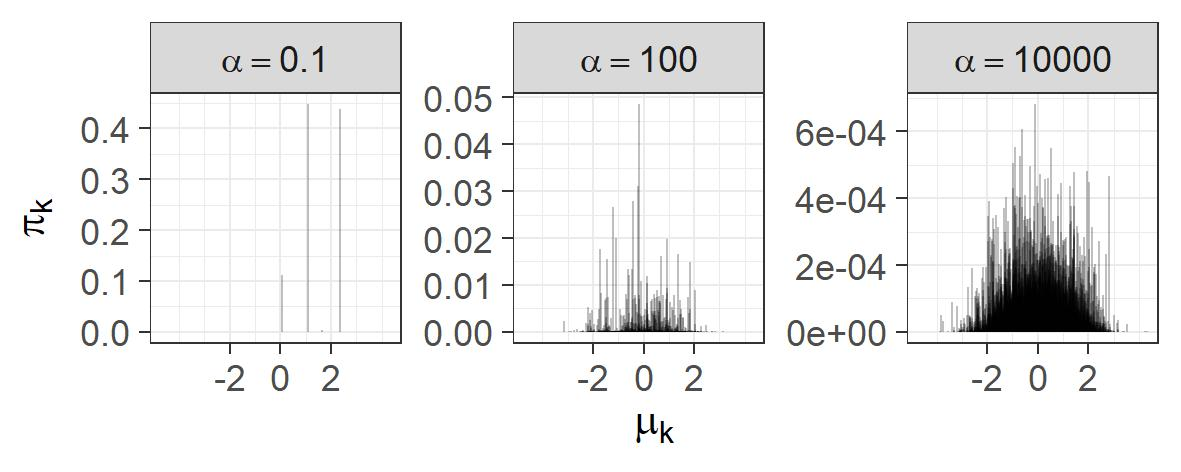
\includegraphics[height=.4\textwidth]{dp1}& \multirowcell{2}{\large $Q=$\\$\alpha=$} & \multirowcell{2}{\large ``prior guess" \\ ``prior sample size"}\\
        \pause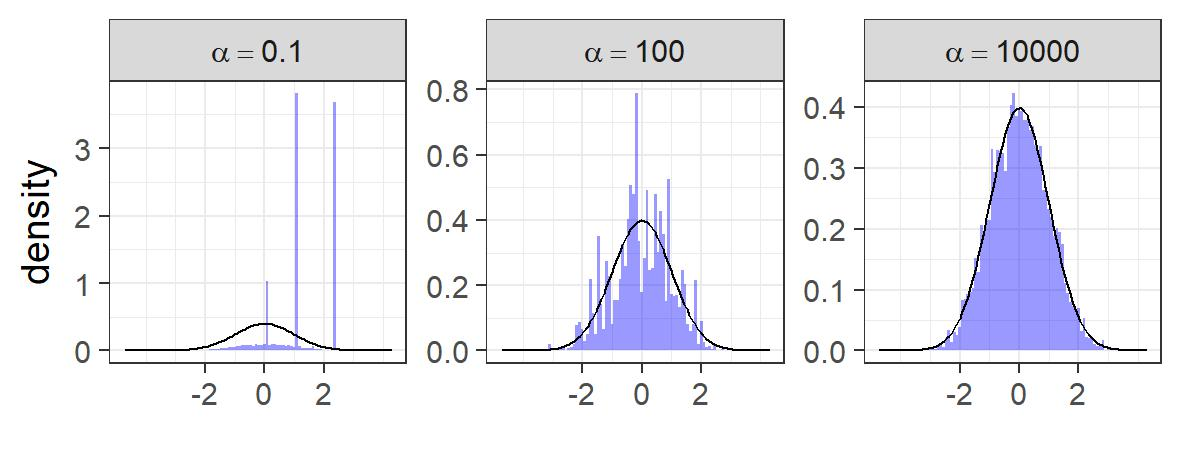
\includegraphics[height=.4\textwidth]{dp2}&&\\
      \end{tabular}
    \end{table}
    \onslide<1->
  }
\end{frame}

\begin{frame}%%[label=current]
  \frametitle{Example: DP mixture}
  {
    \small Suppose we observe $y_{gn};\; g=1,\ldots,200,\; n=1,\ldots,3$ where\\
    \pause\[ y_{gn} \sim \op{N}(\mu_g,\sigma^2),\mbox{ with }\{\mu_g\},\sigma_g\mbox{ unknown.}\]
    \pause $\bar{y}_{g\cdot}$ (unbiased for $\mu_g$) are shown below:\\
    {
      \centering
      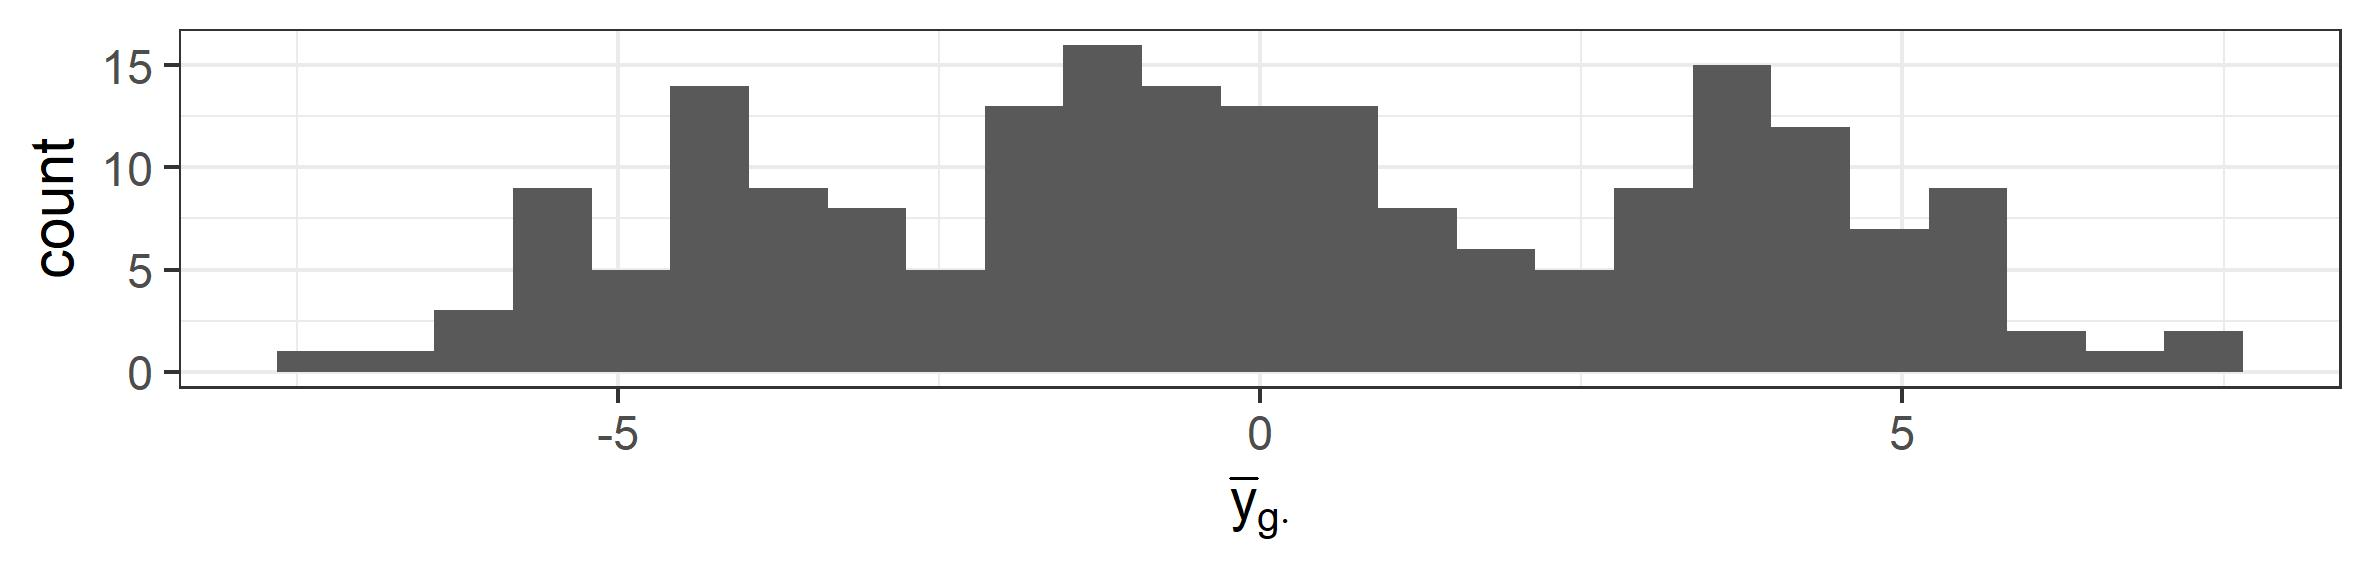
\includegraphics[width=.9\textwidth]{samplemeans_ie}
    }\\
  
    \pause $\mu_g$ were in fact simulated from $1/3\op{N}(-4,1^2) + 1/3\op{N}(0,1^2) + 1/3\op{N}(4,1^2)$.
  }
\end{frame}

\begin{frame}%%[label=current]
  \frametitle{Example: DP as random effects model}
  {
    \footnotesize
    {
      \centering 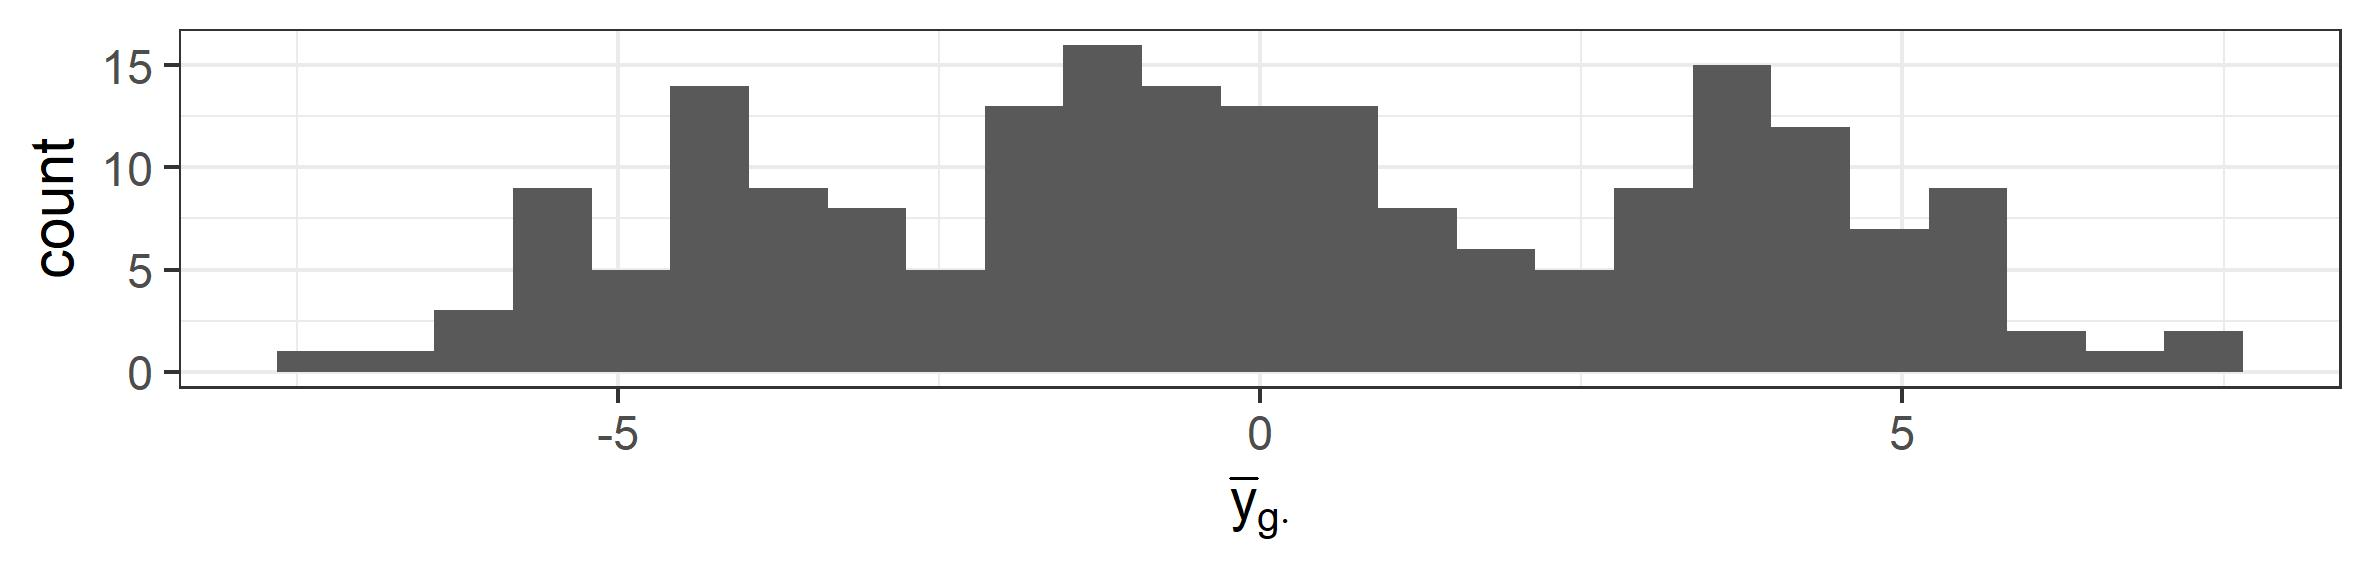
\includegraphics[width=.9\textwidth]{samplemeans_ie}
    }
    Consider these models for $\mu_g$:
    \begin{enumerate}
      \pause \item (Normal) $\mu_g \ind N(\eta, \tau^2)$\\
      with prior distributions $\eta \sim N(0, 5^2)$, $\tau^2 \sim \op{IG}(0.5,0.5)$
      \pause \item (Correct) $\mu_g \ind \pi_1 \op{N}(\eta_1, \tau^2)+\pi_2 \op{N}(\eta_2, \tau^2_2) + \pi_3 \op{N}(\eta_3,\tau^2)$ with prior distributions \\
      $\eta_j \ind N(0,5^2)$, $\tau^2 \sim $\op{IG}(0.5,0.5)$ and $\pi \sim \op{Dir}(1,1,1)$, subject to $\eta_1<\eta_2<\eta_3$.
      \pause \item (DP) $\mu_g \ind \mathcal{P},\; P \sim DP(\alpha Q)$ with $Q \stackrel{d}{=}\op{N}(0,5^2)$, and prior $\alpha \sim \op{Ga}(3,3/14.2)$
    \end{enumerate}
  }
\end{frame}

% \begin{frame}%%[label=current]
% \frametitle{Example - posterior predictive density}
% Can the posterior uncover the true data generating mechanism?\\
% \pause Pointwise intervals for predictive density:
% \begin{enumerate}
% \pause \item (Normal) $p(\mu_{new}|\eta,\tau^2)$ w.r.t. $p(\eta,\tau^2|y)$
% \pause \item (Correct) $p(\mu_{new}|\eta_1,\eta_2,\eta_3,\tau^2)$ w.r.t. $p(\eta_1,\eta_2,\eta_3,\tau^2|y)$
% \pause \item (DP) Posterior draws of $\mathcal{P}$ do not have a density w.r.t. Lebesgue measure \pause ---  instead we use kernel density estimator $\sum_{k=1}^K \pi_k K_h(\mu_{new}-\tilde{\mu}_k)$ w.r.t. $p(\tilde{\mu},\pi|y)$ with a small bandwidth (0.2).
% \end{enumerate}
% \end{frame}

\begin{frame}%%[label=current]
  \frametitle{Example - posterior predictive density}
  \centering
  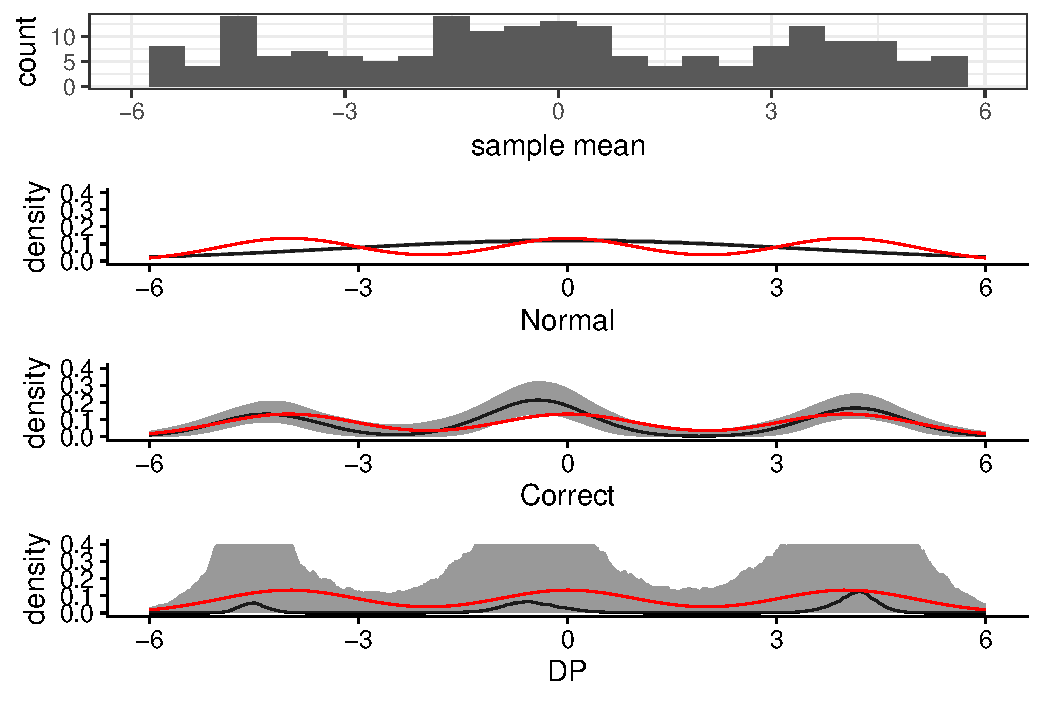
\includegraphics[height=.92\textheight]{predictive_12_5}
\end{frame}

\begin{frame}%%[label=current]
  \frametitle{Posterior CI width and coverage}
  {
    \centering
    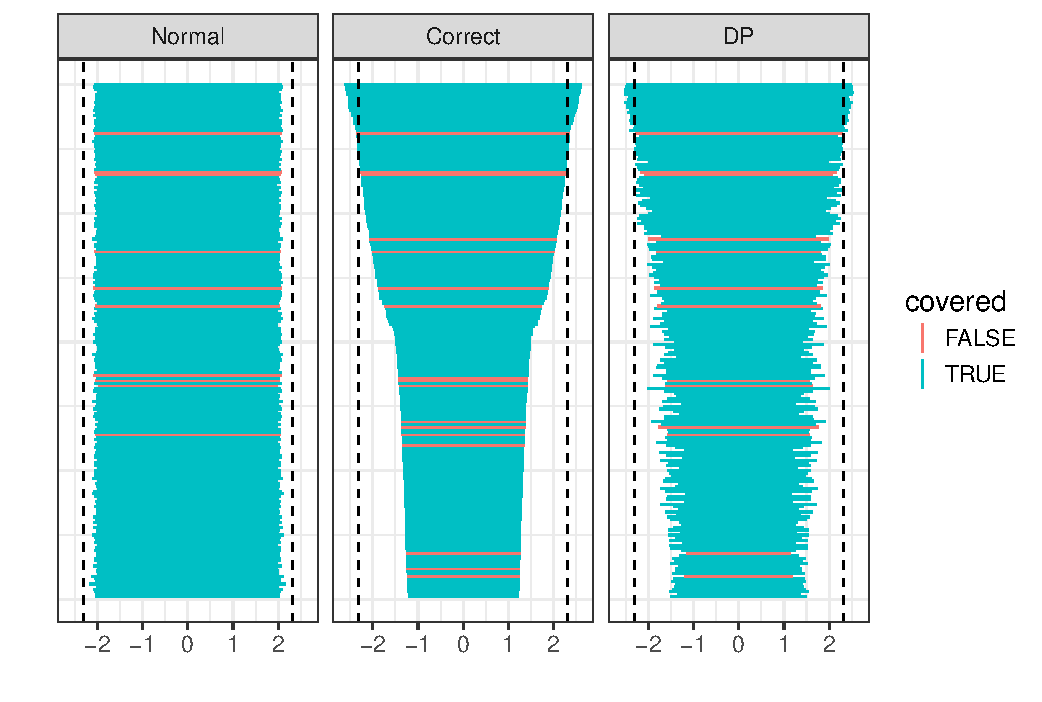
\includegraphics[height=.95\textheight]{cis_12_5}
  }
\end{frame}

\begin{frame}%%[label=current]
  \frametitle{Gene-specific parameter estimates}
  {
    \centering
    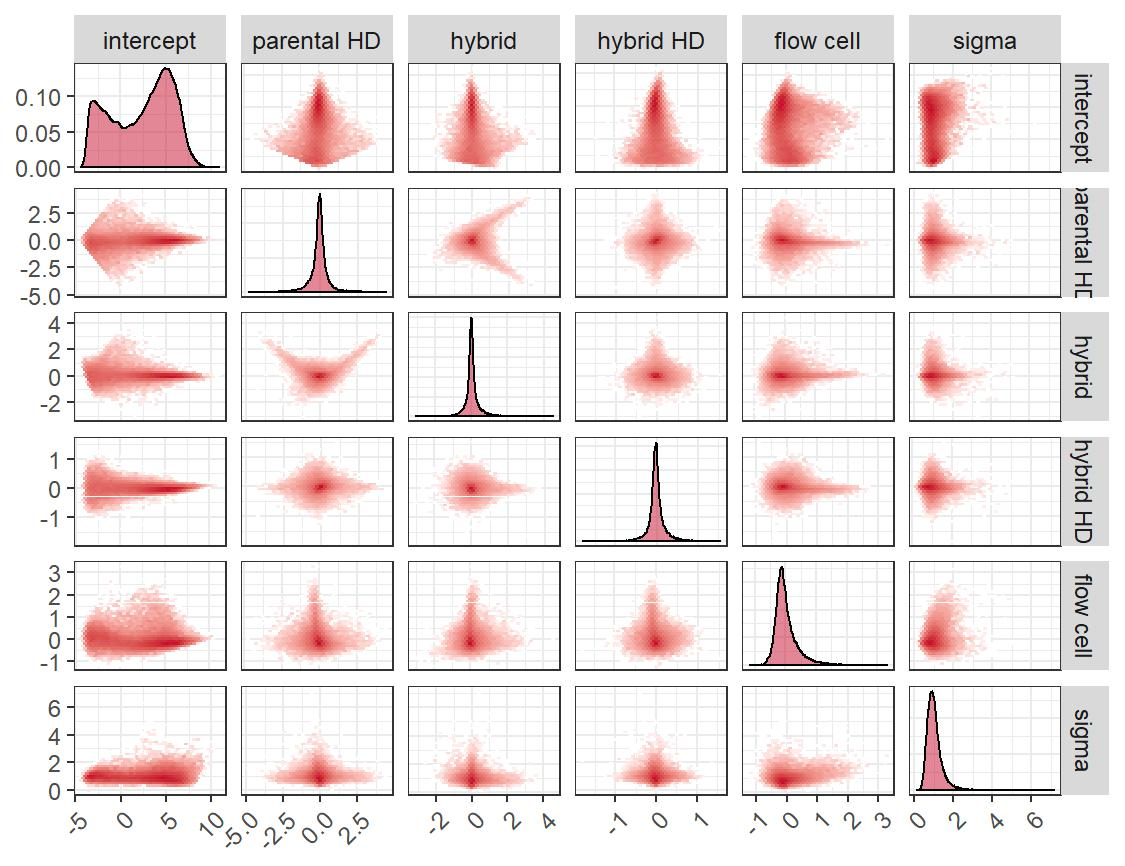
\includegraphics[width=.8\textwidth]{pairs1} \\
  }
\end{frame}

%%%%%%%%%%%%%
\section[BNP model]{BNP model for gene expression}

\begin{frame}%%[label=current]
  \frametitle{BNP model}
  \centering
  \scalebox{.8}{
    \begin{beamerboxesrounded}[upper=upcol,lower=lowcol,shadow=true]{Definitions}
      \[y_{g} \ind \op{N}(X\beta_g, \sigma_g^2W_g^{-1}),\]
      \[(\beta_g^\top,\sigma_g^2) \ind \mathcal{P},\]
      \[\mathcal{P} \sim \op{DP}(\alpha Q),\]
      \pause where
      \begin{itemize}
        \item$y_{g}$ is $N$-vector of log counts per million (log-cpm) for gene $g$
        \pause \item $X$ is the model matrix, with rank $p$,
        \pause \item $W_g$ is a known diagonal matrix of precision weights, $w_{gn}$
      \end{itemize}
    \end{beamerboxesrounded}
    \onslide<1->
  }
\end{frame}

\begin{frame}%%[label=current]
  \frametitle{Dirichlet process (DP)}
  \centering
  \scalebox{.8}{
    \begin{beamerboxesrounded}[upper=upcol,lower=lowcol,shadow=true]{Stick-breaking representation \citep{sethuraman}:}
      $\mathcal{P} \sim \op{DP}(\alpha Q)$ \pause $\implies$
      \begin{itemize}
        \item $\mathcal{P} \stackrel{d}{=} \sum_{k=1}^\infty \pi_k \delta_{(\tilde{\beta}_k^\top,\tilde{\sigma}^2_k)},\quad$ where $\delta_{}$ is the Dirac delta function \pause with
        \item $(\tilde{\beta}_k^\top,\tilde{\sigma}^2_k) \ind Q$ \pause and
        \item $\nu_k = \frac{\pi_k}{1-\sum_{\ell<k} \pi_\ell} \ind \op{Be}(1,\alpha)$, $k<K-1$.
        \item $\nu_K = 1 \implies \pi_\ell =0$ for $\ell>K$.
        \pause \item Define $\zeta_g \in \{1,\ldots,K\}$, so $(\beta_g^\top,\sigma_g) = (\tilde{\beta}_{\zeta_g},\tilde{\sigma}_{\zeta_g}^2)$ \pause so that
        \item $\zeta_g \ind \op{Categorical}(\pi_1,\ldots,\pi_K)$ \pause and
        \item $y_g \ind \op{N}(X\tilde{\beta}_{\zeta_g},\tilde{\sigma}_{\zeta_g}^2 W_g^{-1})$. 
      \end{itemize}
    \end{beamerboxesrounded}
    \onslide<1->
  }
\end{frame}

\begin{frame}%%[label=current]
  \frametitle{Prior distibution for $\alpha$}
    \begin{columns}
    \begin{column}{.5\textwidth}
      {\footnotesize 
      \begin{itemize}
        \pause \item $U=$ number of unique $\zeta_g$
        \pause \item $\op{E}(U) = \sum_{g=1}^G \alpha/(g + \alpha - 1)$.
        \pause \item Prior for $\alpha$: $\alpha \sim \op{Ga}(3,3/G^{0.5})$
      \end{itemize}
      }
      \onslide<1->
    \end{column}
    \begin{column}{.65\textwidth}
      \begin{figure}
        \centering
        \includegraphics[height=.75\textheight]{alphaprior}
      \end{figure}
    \end{column}
  \end{columns}
\end{frame}

\begin{frame}%%[label=current]
  \frametitle{Selection of $Q$}
  $Q \stackrel{d}{=} \prod_{\ell=1}^p\op{N}(m_\ell,c^2_\ell)\times\op{IG}(a_\sigma,b_\sigma)$\\
  
  \vspace{.5cm}
  
  \begin{itemize}
    \pause \item $m_\ell$, $c^2_\ell$, $a_\sigma$, $b_\sigma$ selected to roughly match marginal distributions of unpooled estimates of $\beta_g$, $\sigma_$
    \pause \item Conditional conjugacy for $\tilde{\beta}_k,\; \tilde{\sigma}_k^2$
    \pause \item Diffuse distributions would lead to inefficient posterior sampling
  \end{itemize}
\end{frame}

\begin{frame}%%[label=current]
  \frametitle{Directed acyclic graph (DAG)}
  \centering
  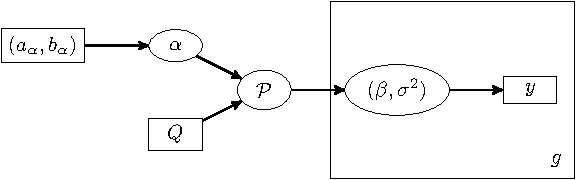
\includegraphics[width=\textwidth]{my_dag_small0}
\end{frame}

\begin{frame}%%[label=current]
  \frametitle{DAG with augmented data}
  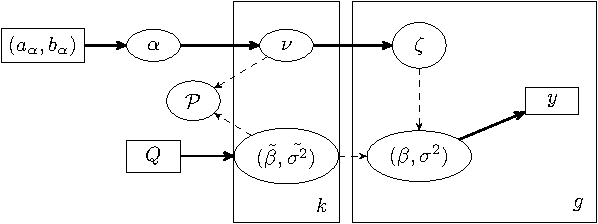
\includegraphics[width=\textwidth]{my_dag_small}
\end{frame}

\begin{frame}%%[label=current]
  \frametitle{Full conditionals}
  \begin{beamerboxesrounded}[upper=upcol,lower=lowcol,shadow=true]{Gibbs sampler}
    \begin{enumerate}
      \item Draw $\alpha$, $\zeta_g$
      \item Draw $\pi$
      \item Draw $\tilde{\beta}_k$
      \item Draw $\tilde{\sigma}_k$
    \end{enumerate}
  \end{beamerboxesrounded}
\end{frame}

\begin{frame}%%[label=current]
  \frametitle{Full conditionals}
  1. Draw $\alpha$, $\zeta_g$ (conditionally independent):\\
  
  \[\alpha \sim \op{Gamma}(K + a_\alpha - 1, -\log \pi_K + b_\alpha)\]
  
  \[\zeta_g \ind \op{Categorical}\left(\hat{\pi}_{g1},\ldots,\hat{\pi}_{gK} \right),\]
  with
  \[\hat{\pi}_{gk} \propto \pi_k \op{N}\left( y_g;X\tilde{\beta}_k,\tilde{\sigma}_k^2 W_g^{-1} \right)\]
\end{frame}

\begin{frame}%%[label=current]
  \frametitle{Full conditionals}
  2. Draw $\pi$
  
  \[\nu_k \ind \op{Be}(M_k + 1, \sum_{\ell>k}M_\ell + \alpha); k < K,\]
  where $M_k$ is the number of $\zeta_g$ equal to $k$.
  
  Then $\pi_k = \nu_k \prod_\ell<k(1-\nu_k$.
\end{frame}

\begin{frame}%%[label=current]
  \frametitle{Full conditionals}
  3. Draw $\tilde{\beta}_k$ (conditionally independent)
  
  \[\tilde{\beta}_k \ind \op{N}(\hat{m}_k,\, \hat{C}_k),\]
  where
  \[\hat{C}_k= \left( \tilde{\sigma}^{-2}_g\sum_{g:\zeta_g=k}
    X^\top W_g X + C^{-1} \right)^{-1},\]
  \[\mbox{ and }\hat{m}_k=\hat{C}_k \left(\sum_{g:\zeta_g=k} X^\top W_g y_g +
        C^{-1}m \right)\]
\end{frame}

\begin{frame}%%[label=current]
  \frametitle{Full conditionals}
  4. Draw $\tilde{\sigma}_k^2$ (conditionally independent)
  
  \[\tilde{\sigma}_k^2 \ind \op{IG}(\hat{a}_k,\hat{b}_k),\]
  where
  \[\hat{a}_k = a_{\sigma^2} + \frac{1}{2}NM_k,\mbox{ and }\]
  \[\hat{b}_k= b_{\sigma^2} + \frac{1}{2}\sum_{g:\zeta_g=k}y_g^\top W_g y_g -2 \beta_g^\top X^\top W_g y_g  +\beta_g^\top X^\top W_g X \beta_g\]
\end{frame}


\begin{frame}%%[label=current]
  \frametitle{Counts to log-cpm + precision weights (voom)}
  \centering
  \scalebox{.8}{
    \begin{beamerboxesrounded}[upper=upcol,lower=lowcol,shadow=true]{Definitions}
      \pause\[\tilde{r}_g = \frac{1}{N}\sum_{n=1}^N y_{gn} + \log_2(\tilde{R}) - \log_2(10^6)\]
      \pause\[s_g = \sqrt{MSE}\mbox{ from ind. OLS fits of, }y_g \sim N(X\beta_g, \sigma^2_gI_{n\timesn})\]
      \onslide<1->
      \citep{voom}  
    \end{beamerboxesrounded}
  }
\end{frame}

\begin{frame}%%[label=current]
  \frametitle{Mean-variance trend}
  \only<1>{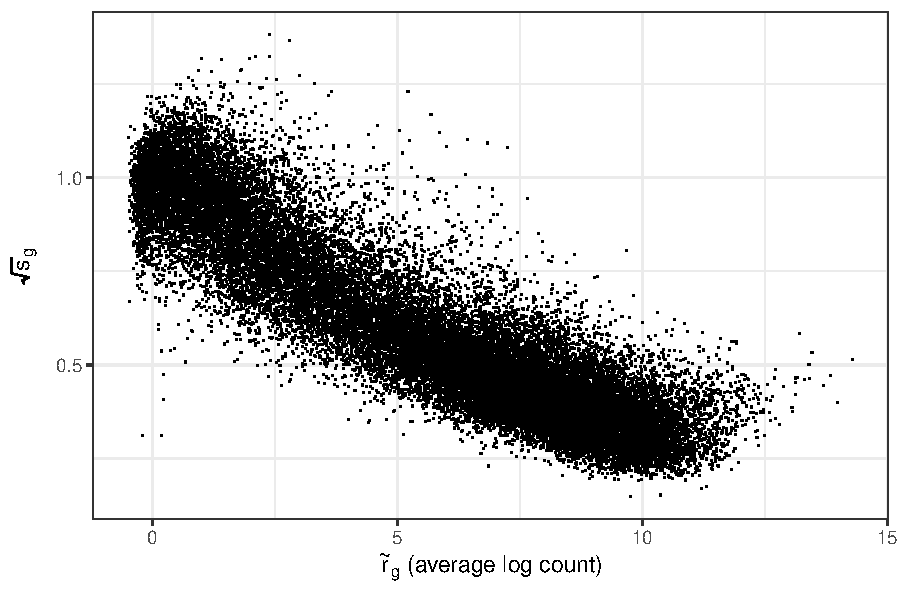
\includegraphics[width=\textwidth]{voom1}}
  \only<2>{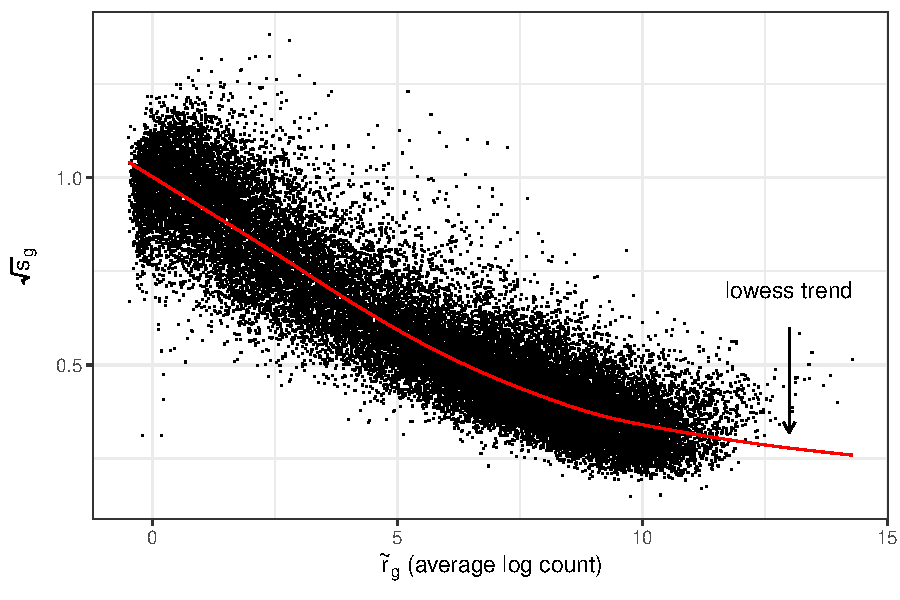
\includegraphics[width=\textwidth]{voom2}}
\end{frame}

\begin{frame}%%[label=current]
  \frametitle{Variance modeling at the observation level}
  \centering
  \scalebox{.8}{
    \begin{beamerboxesrounded}[upper=upcol,lower=lowcol,shadow=true]{Definitions}
      \[\tilde{r}_g = \frac{1}{N}\sum_{n=1}^N y_{gn} + \log_2(\tilde{R}) - \log_2(10^6)\]
      \[s_g = \sqrt{MSE}\mbox{ from ind. OLS fits of, }y_g \sim N(X\beta_g, \sigma^2_gI_{n\timesn})\]
      \pause \[\lambda_{gn} = x_{n}\hat{\beta}_g + \log_2(R_n) - \log_2(10^6)\]
      \pause \[w_{gn} = \widehat{lowess}(\lambda_{gn})\]
      \onslide<1->
      \citep{voom}  
    \end{beamerboxesrounded}
  }
\end{frame}
%%%%%%%

\section{Computation}

\begin{frame}%[label=current]
  \frametitle{GPU computing}
  \begin{itemize}
    \item Scientific programming APIs have been developed for GPUs
    \item GPUs offer a higher degree of parallelism with lower latency than parallel CPU computing
    \item The utility of switching to GPUs is problem dependent:
    \begin{itemize}
      \item The task must be broken into identical problems of similar size (preferably independent)
      \item There must be enough of these to occupy most of the GPU
      \item Typically requires more time to develop code
    \end{itemize}
  \end{itemize}
\end{frame}

\begin{frame}%[label=current]
  \frametitle{Implementation overview}
  \texttt{R} $\rightarrow$ \texttt{C++} $\rightarrow$ \texttt{CUDA}
  \begin{itemize}
    \pause\item Parallel updates are performed on conditionally independent model parameters
    \pause\item Prerequisite computations are accelerated by the use of
    \begin{itemize}
      \pause\item Parallel reductions
      \pause\item Parallel scans
      \pause\item Optimized linear algebra routines, both global (large matrix multiplication) and multi-threaded (solving linear systems)
      \pause\item Custom multi-threaded operations (ex. Cholesky decomposition)
    \end{itemize}
  \end{itemize}
\end{frame}

\begin{frame}%[label=current]
  \frametitle{Example: update $\zeta_g$}
  Outcome: Overwrite current value of $\zeta_g$ with new values drawn from their full conditionals, i.e. $\op{Categorical}(\hat{\pi}_{g1},\ldots,\hat{\pi}_{gK})$.
  
  \vspace{.7cm}
  Outline of GPU implementation:
  \small
  \begin{enumerate}
    \pause\item Compute $\{\hat{\pi}\}_{G\times K}$
    \pause\item Compute scans (cumulative sums), $(S_{g1},\ldots,S_{gK});\;g=1,\ldots,G$ (parallel across $(g,k)$.)
    \pause\item Generate $U_g \sim \op{U}(0,1);\;g=1,\ldots,G$. Scale by $S_{gK}$ (across $g$.)
    \pause\item Define $D_{gk} \in \{0,1\};\;k=1,\ldots,K-1$ and set it to $1$ if $S_{gK}U_g > S_{gk}$, $0$ otherwise (across $(g,k)$.)
    \pause\item Reduce by $g$ (sum) the $D_{gk}$, i.e. $\zeta_g \leftarrow \sum_{k=1}^{K-1} D_{gk}$.
    %\item draw_zeta
    %\item weights
    %\item mulinomial draw
  \end{enumerate}
\end{frame}

\begin{frame}[label=current]
  \frametitle{Parallel scan}
  \begin{figure}
    \centering
    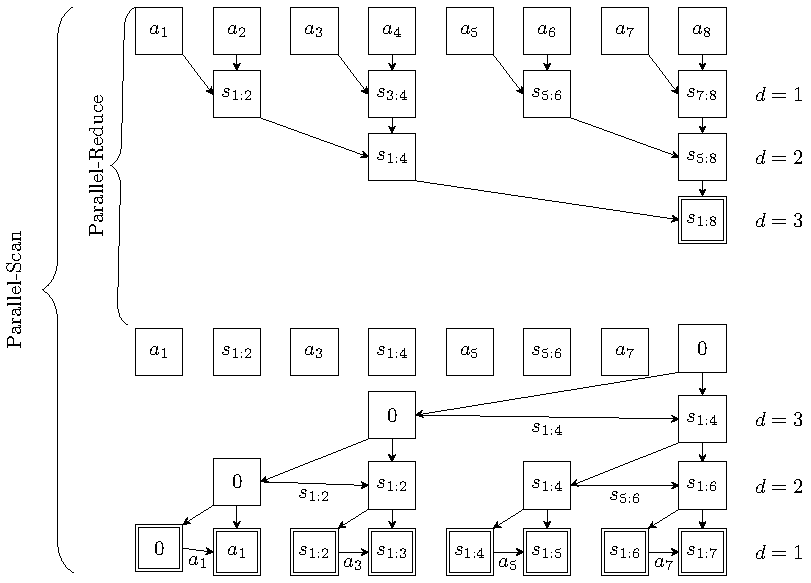
\includegraphics[height=.8\textheight]{CopyOfdiagram}\\
    {
      \scriptsize \citep{blelloch1990}
    }
  \end{figure}
\end{frame}
\begin{frame}%[label=current]
  \frametitle{Evaluation of running time}
  Critical question: On average, how long to get one effective sample?
  
  Simulation study:
  \begin{itemize}
    \item Dimensions manipulated: G, K, p
    \item $\tilde{\beta}_{k\ell}$ from independent normals (variance decreasing in $p$, $\tilde{\sigma}^2_k$ independent from inverse gamma, $k=1,\ldots,K_t = G^{0.5}$.
    \item $\zeta_g \sim \op{Categorical}\left(\pi_1=1/K_0,\ldots,\pi_{K_0}=1/K_0 \right);\; y_g \sim N(X\beta_{\zeta_g}, \sigma^2_{\zeta_g})$.
    \item Chose to focus on $\alpha$, whose autocorrelation is high relative to gene-specific parameters.
  \end{itemize}
\end{frame}

\begin{frame}%[label=current]
  \frametitle{Running time - simulation study}
  \includegraphics[width=\textwidth]{comb-timing}
\end{frame}

\begin{frame}%[label=current]
  \frametitle{Running time - simulation study}
  % Results of fitting 
  % \[\log_2(\mbox{seconds}) = \mbox{intercept} + \log_2(K)\gamma_1 +  \log_2(G)\gamma_2 +  \log_2(p)\gamma_3 + \epsilon,\]
  % \[\op{E}(\epsilon)=0$\]
  % \centering
  \begin{table}
    \centering
    \begin{tabular}{ccccc}
      \hline
      factor &mult. effect& Est. & lower 95\% & upper 95\% \\ 
      \hline
      K & $2^{\gamma_1}$ & 3.3 & 2.8 & 3.8 \\ 
      G & $2^{\gamma_2}$ & 1.2 & 1.0 & 1.4 \\ 
      p & $2^{\gamma_3}$ & 0.5 & 0.4 & 0.6 \\ 
      \hline
    \end{tabular}
  \end{table}

\end{frame}

\section[Case study]{Case study: Heterosis in \citet{paschold}}

% \begin{frame}
%   \frametitle{Simulation studies - overview}
%   Objectives:
%   \begin{enumerate}
%     \item Comparison to non-hierarchical log-linear method:
%     \begin{itemize}
%       \pause \item Demonstrate utility of hierarchical model under favorable conditions
%       \pause \item Ignore impact of voom procedure
%     \end{itemize}
%     \pause \item Comparison to count-based methods:
%     \begin{itemize}
%       \pause \item Establish competitiveness under fair conditions
%     \end{itemize}
%   \end{enumerate}
% \end{frame}

\begin{frame}
  \frametitle{Comparison to non-hierarchical log-linear method}
  \begin{itemize}
    \item Conditionally normal data, true parameters distributed by posterior realization of $\mathcal{P}$ from BNP analysis of \citet{paschold} data
    \item 10 simulations, 10,000 genes each
    \item Modes of comparison:
    \begin{itemize}
      \item Ranking of genes by treatment effect larger than a threshold (TREAT) using ROC, AUC
      \item Mean squared error in point estimates for each coefficient component
    \end{itemize}
    \item Competing method: \texttt{limma} \citep{mccarthy}
    \begin{itemize}
      \item ``linear modeling of microarrays"
      \item Uses empirical Bayes shrinkage of $\sigma^2_g$ in computing t-statistic
    \end{itemize}
  \end{itemize}
\end{frame}

\begin{frame}
  \frametitle{TREAT}
  \begin{itemize}
    \pause\item Test hypothesis that an effect exceeds a threshold, i.e., $H_{g\ell}: |\beta_{g \ell}|>\tau$
    \pause\item p-value reported is upper bound for p-values, based on value in null parameter space closest to observed estimate of $\beta_{g\ell}$
    \pause\item Point is to focus on biologically meaningful differences
    \pause\item No specific threshold is recommended; values ranging from 0.15-1 are mentioned in the paper
  \end{itemize}
  \onslide<1->
  \citep{treat}
\end{frame}

\begin{frame}
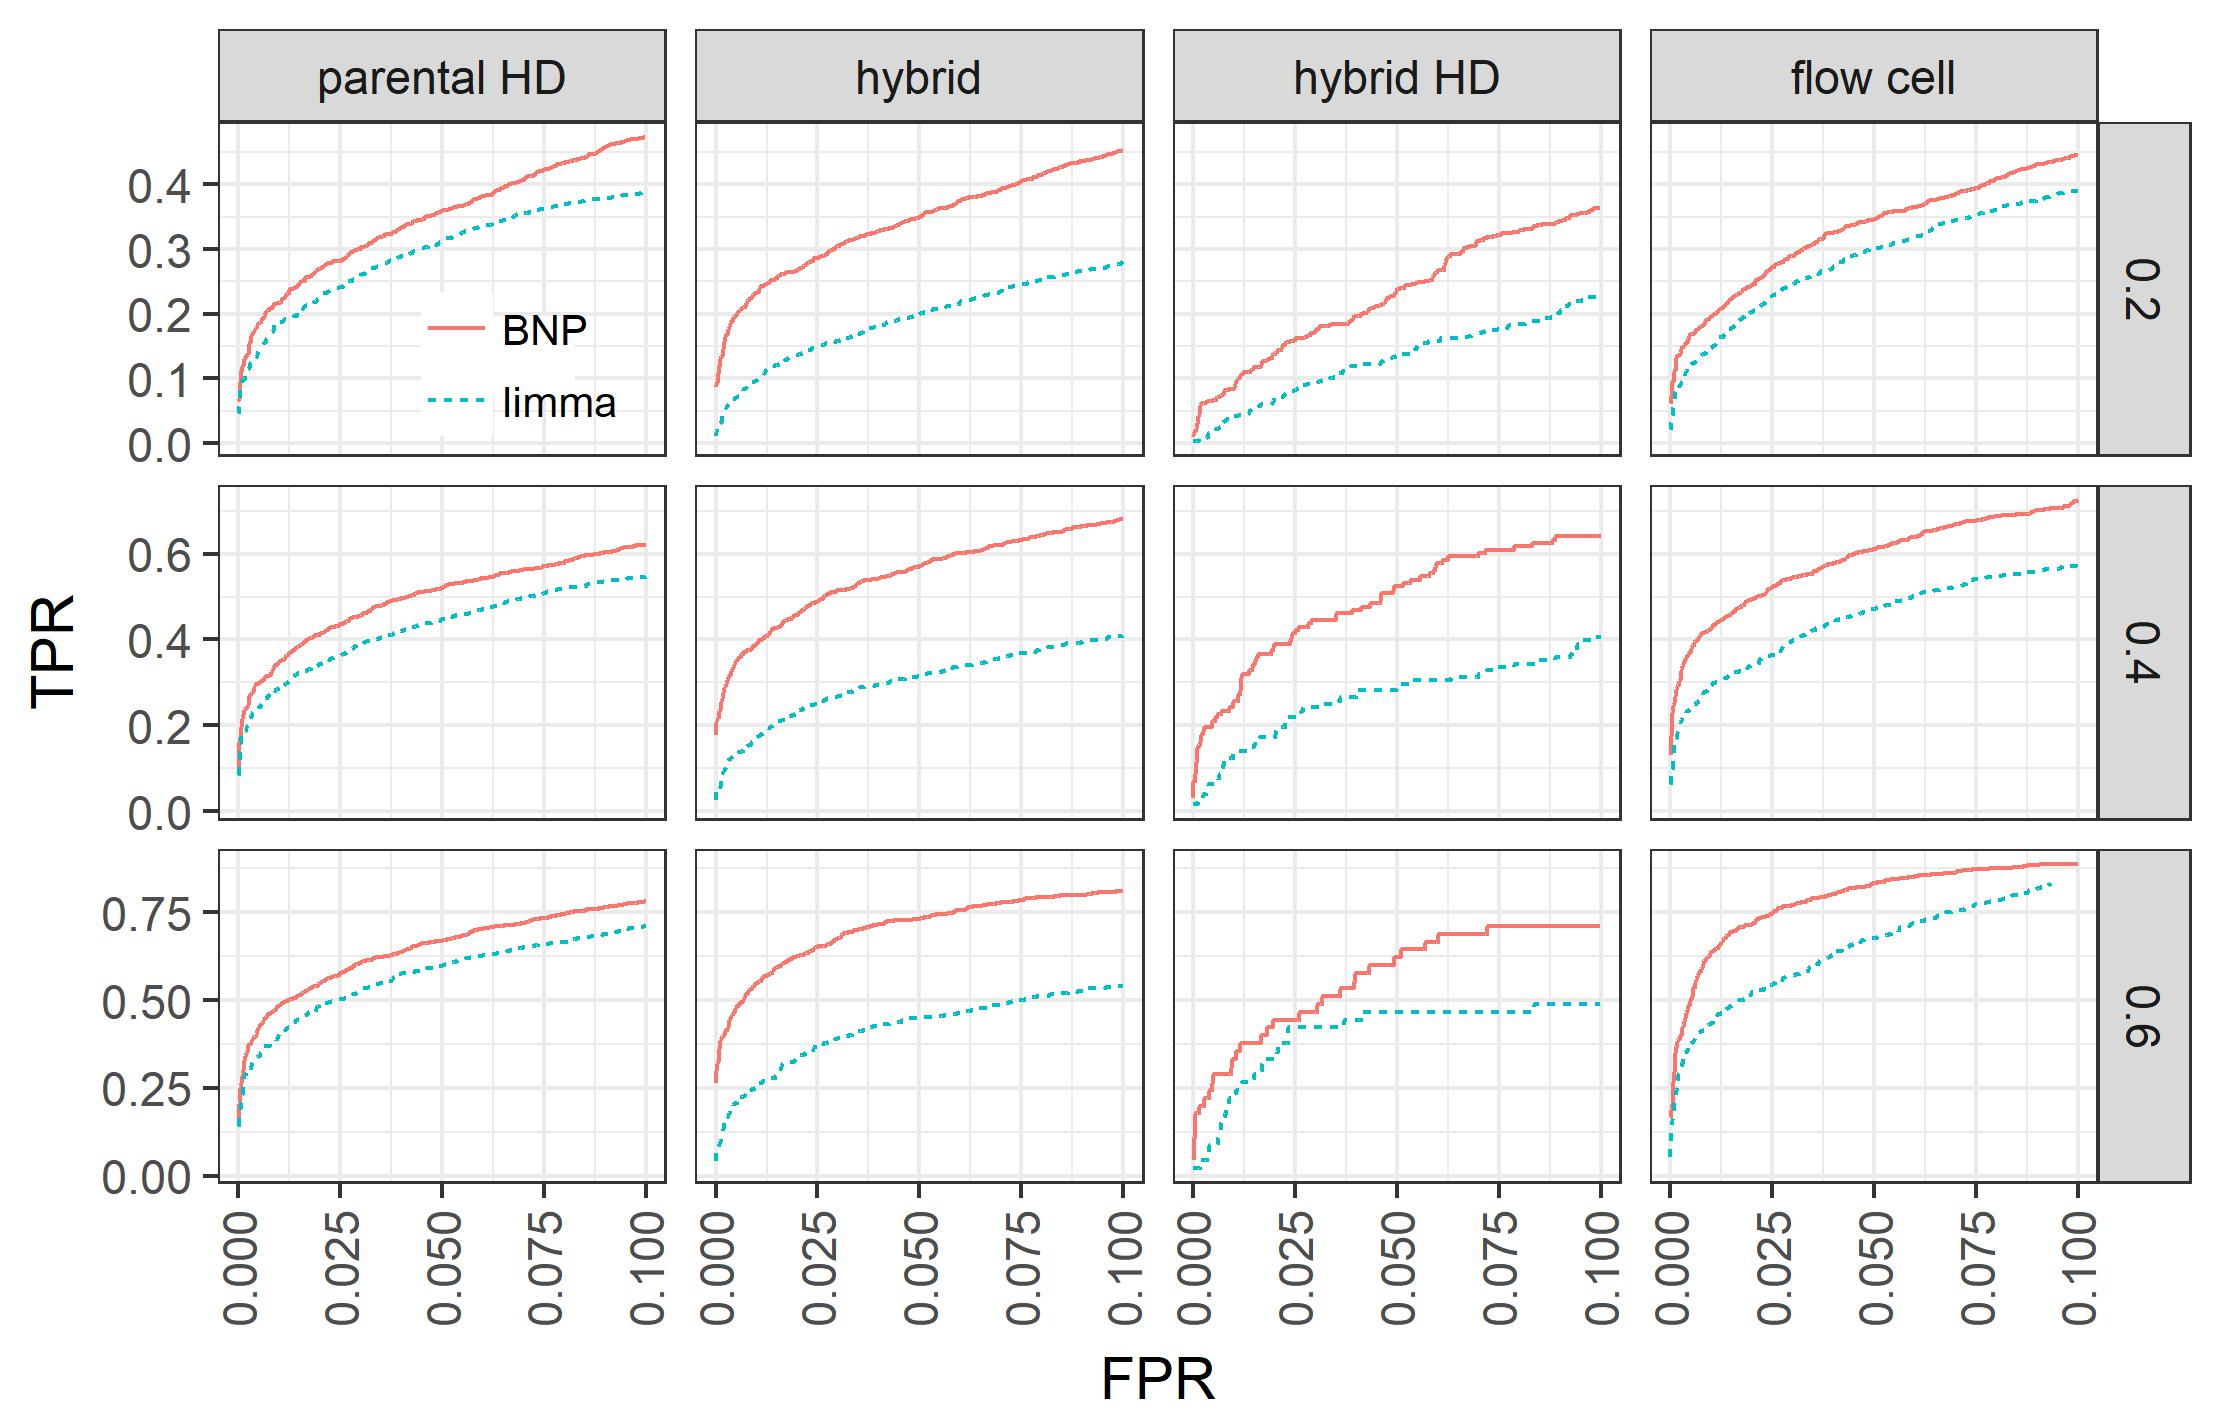
\includegraphics[width=\textwidth]{ss1-roc}
\end{frame}

\begin{frame}
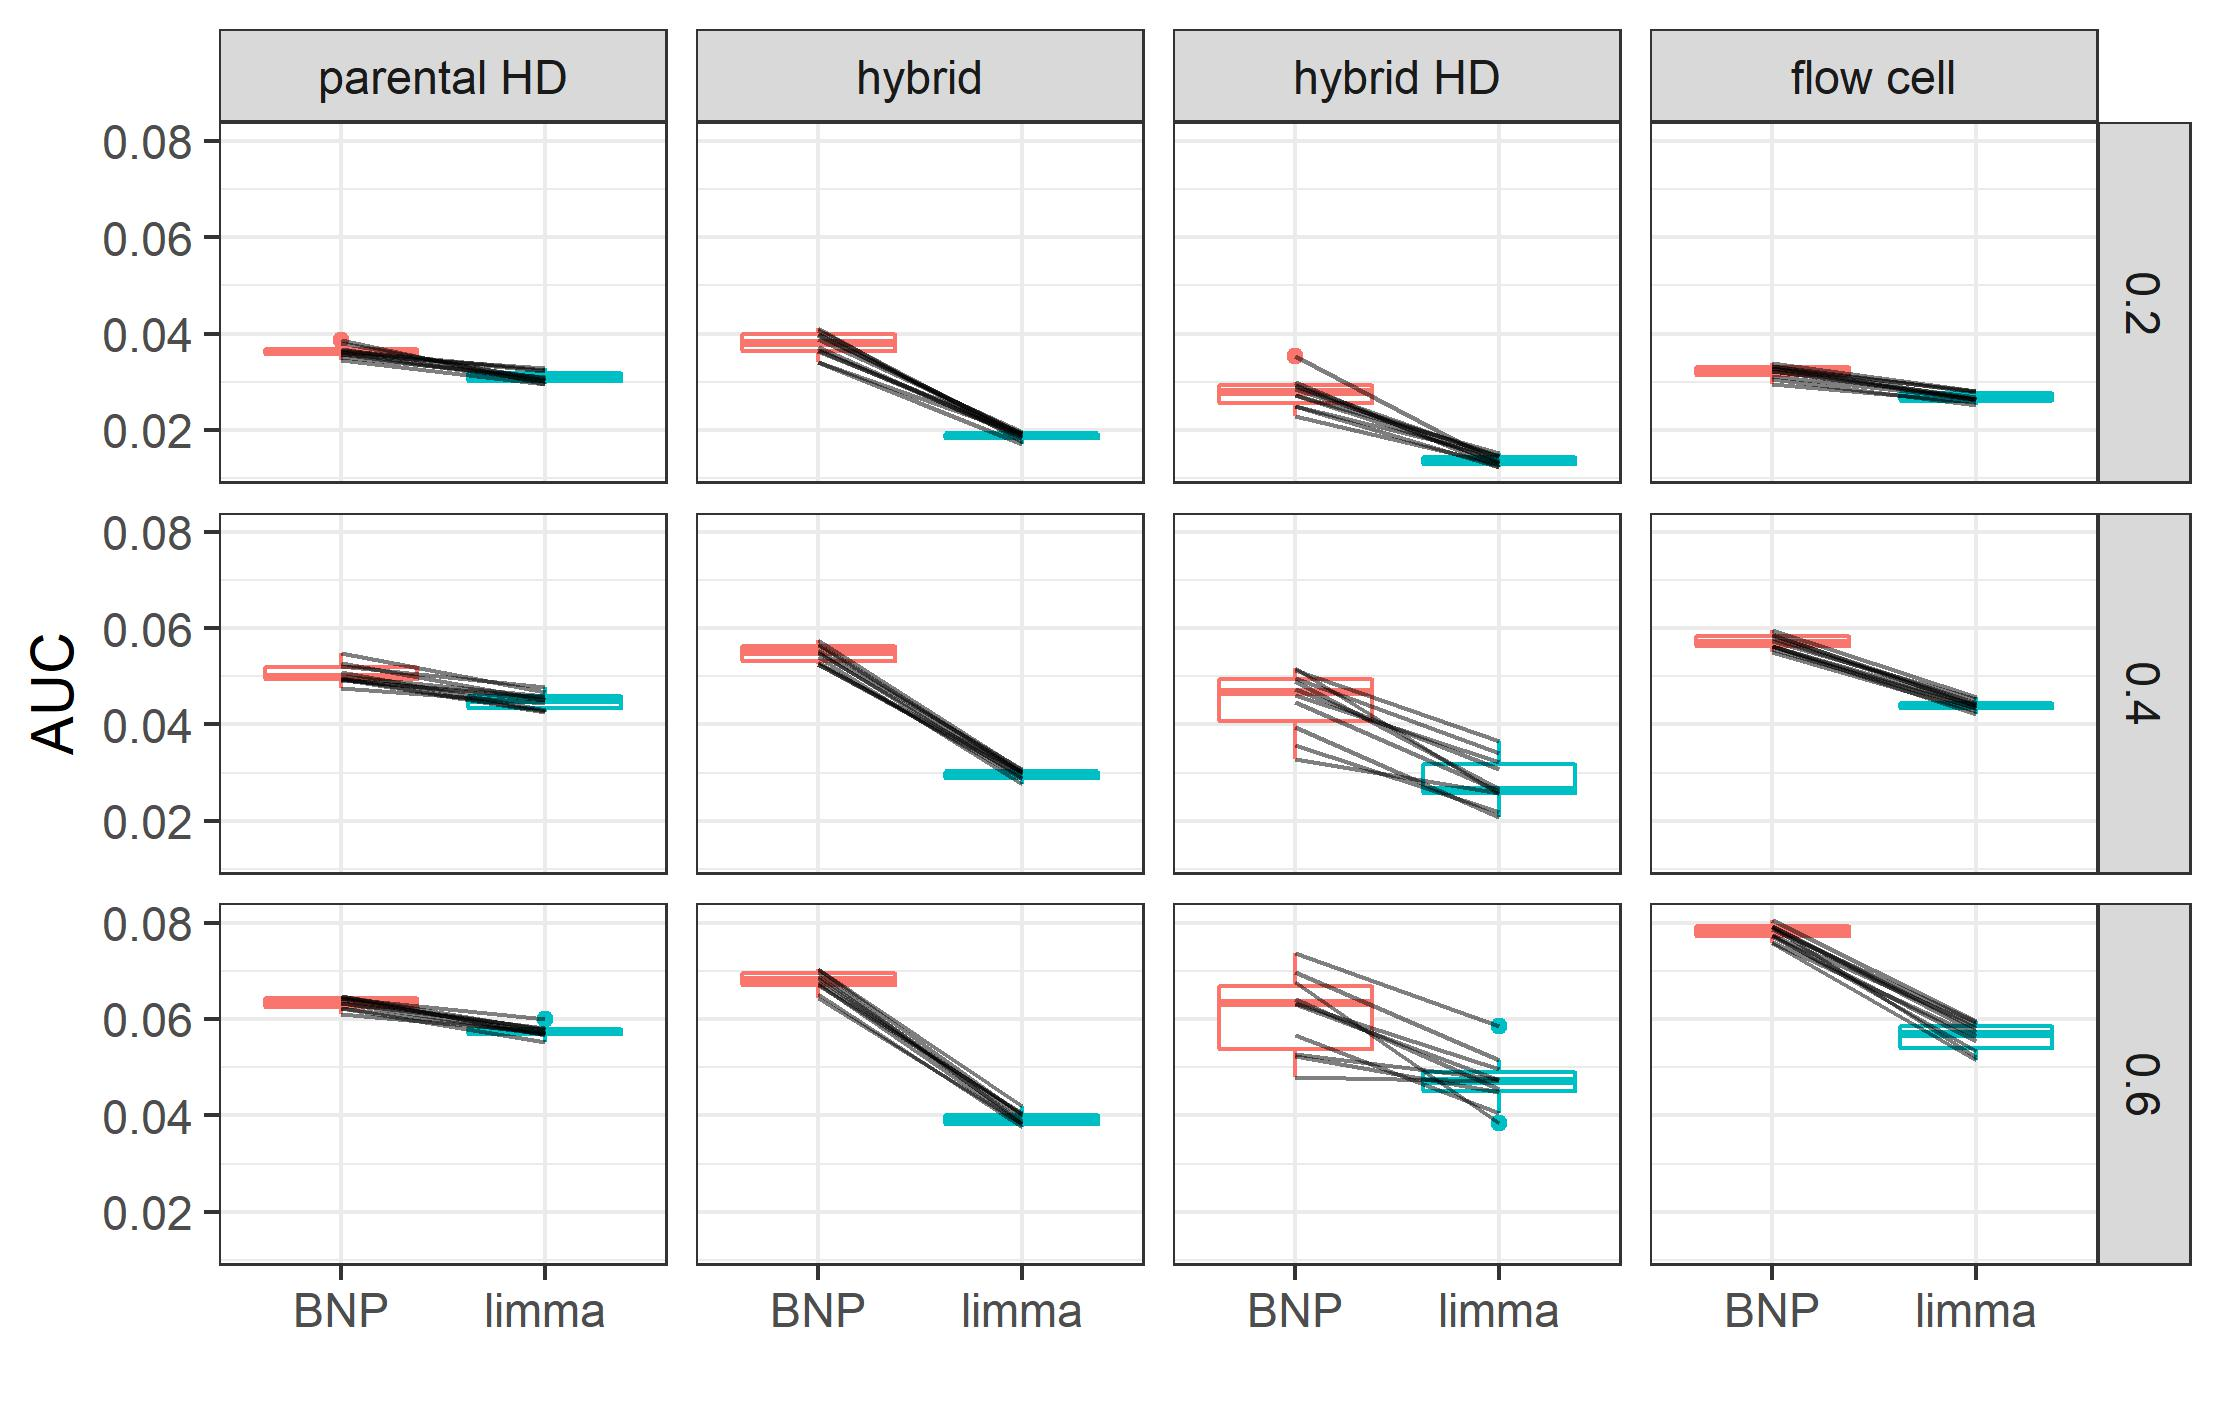
\includegraphics[width=\textwidth]{ss1-auc}
\end{frame}

\begin{frame}[label=current]
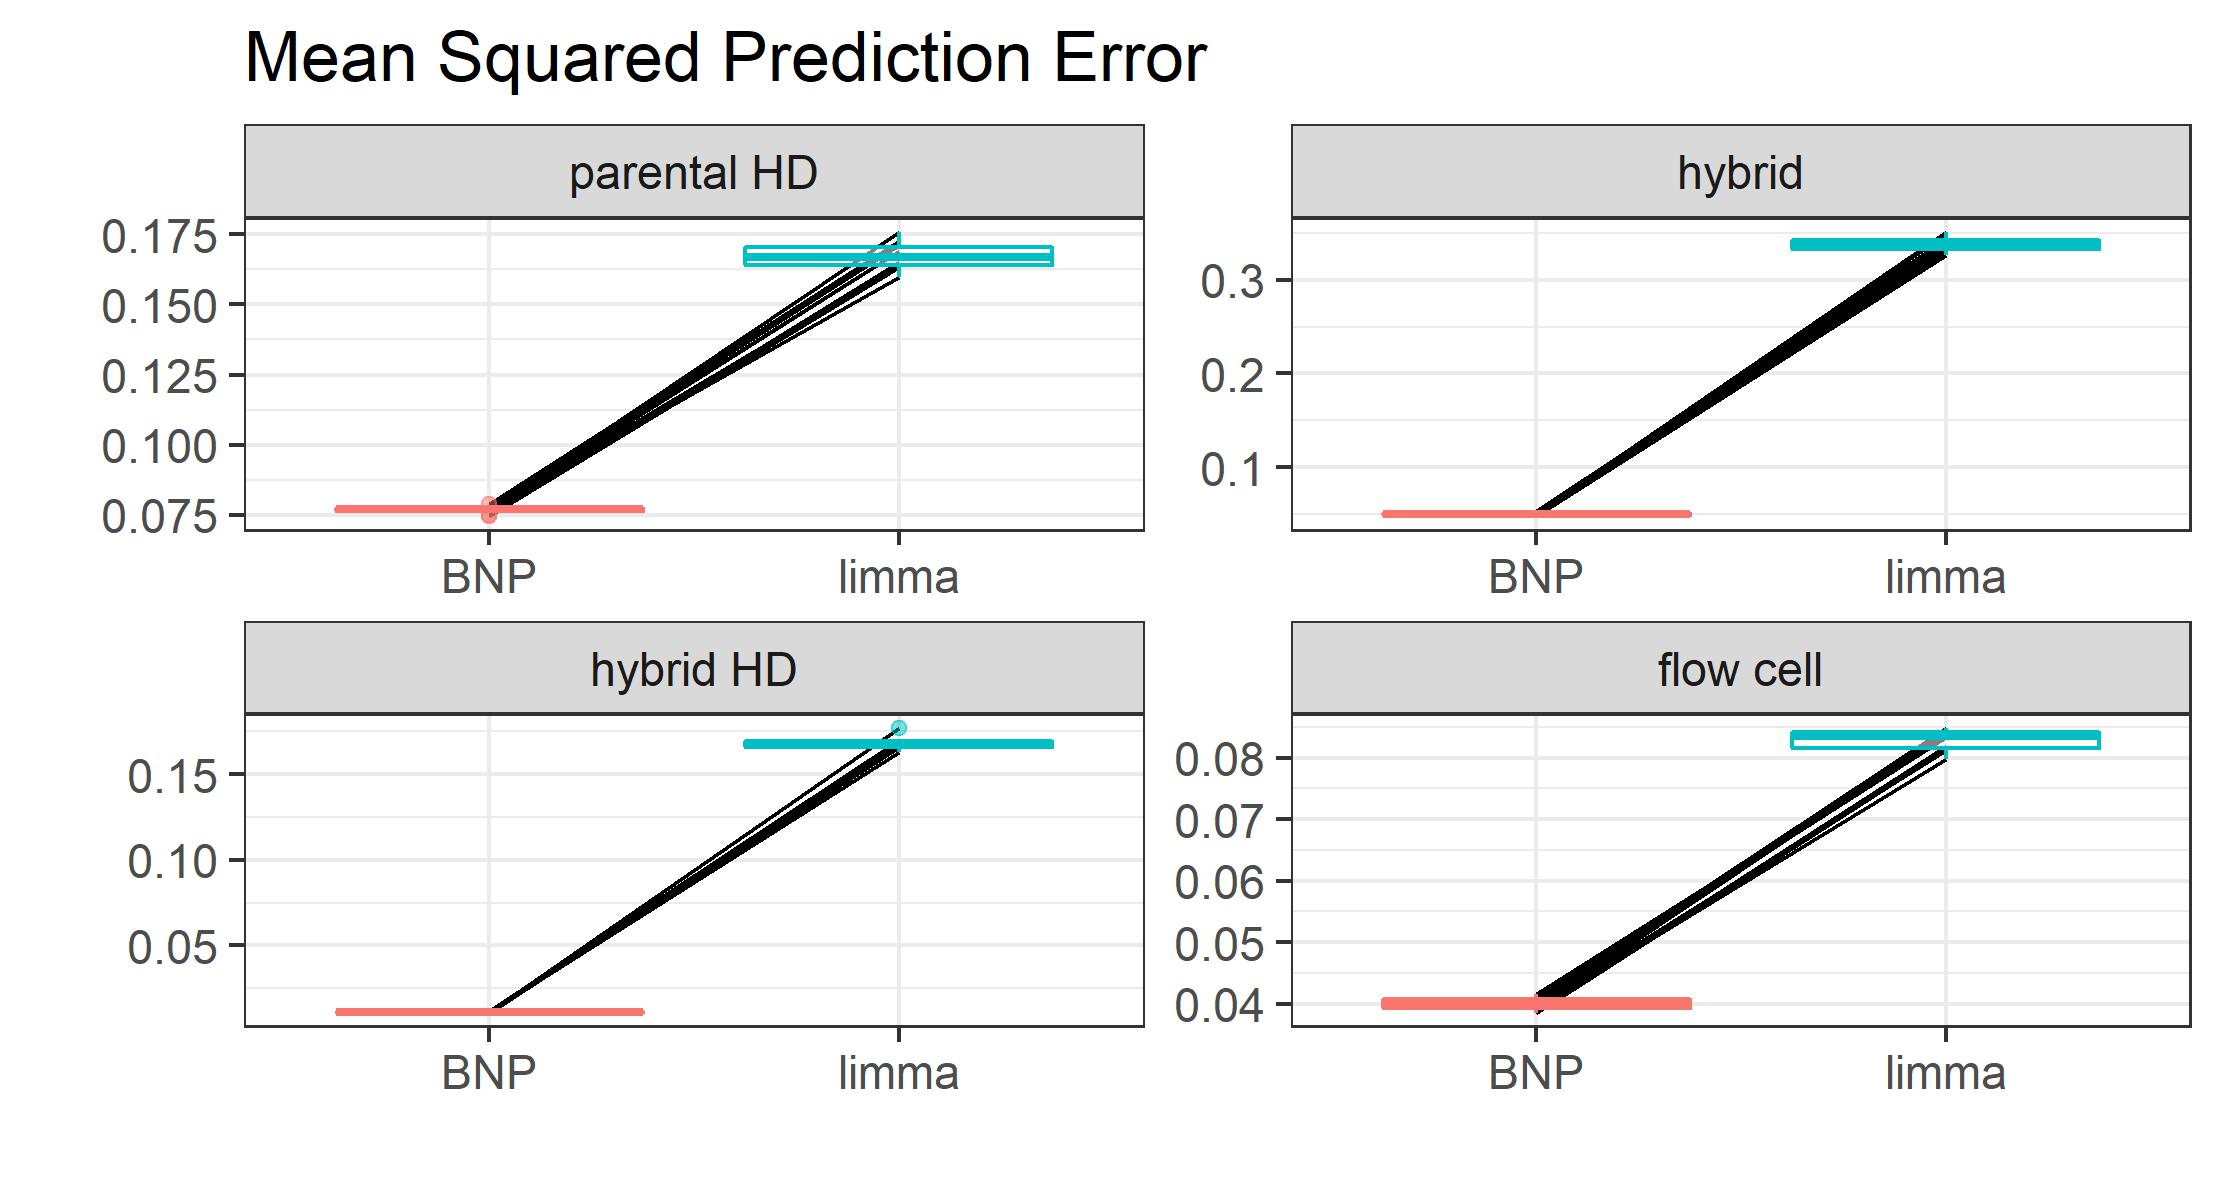
\includegraphics[width=\textheight]{ss1-mspe}
\end{frame}

\begin{frame}
  \frametitle{Comparison to count-based methods}
  \begin{itemize}
    \item Conditionally normal log-cpm, true parameters determined by point estimates of \citet{paschold} data using voom-limma (including estimated precisions)
    \item Transformed and rounded to produce "counts"
    \item 10 simulations, 10,000 genes each
    \pause\item Modes of comparison:
    \begin{itemize}
      \pause\item Ranking of genes by treatment effect larger than a threshold (TREAT) using ROC, AUC
      \pause\item Mean squared error in point estimates for each coefficient component
    \end{itemize}
    \pause\item Competing methods:
    \begin{itemize}
      \pause\item \texttt{edgeR} (defaults) \citep{edger2010}
      \pause\item \texttt{DESeq2} (defaults) \citep{deseq2014}
      \pause\item \texttt{DESeq2} (using shrinkage prior on $\beta$)
    \end{itemize}
  \end{itemize}
\end{frame}

\begin{frame}[label=current]
  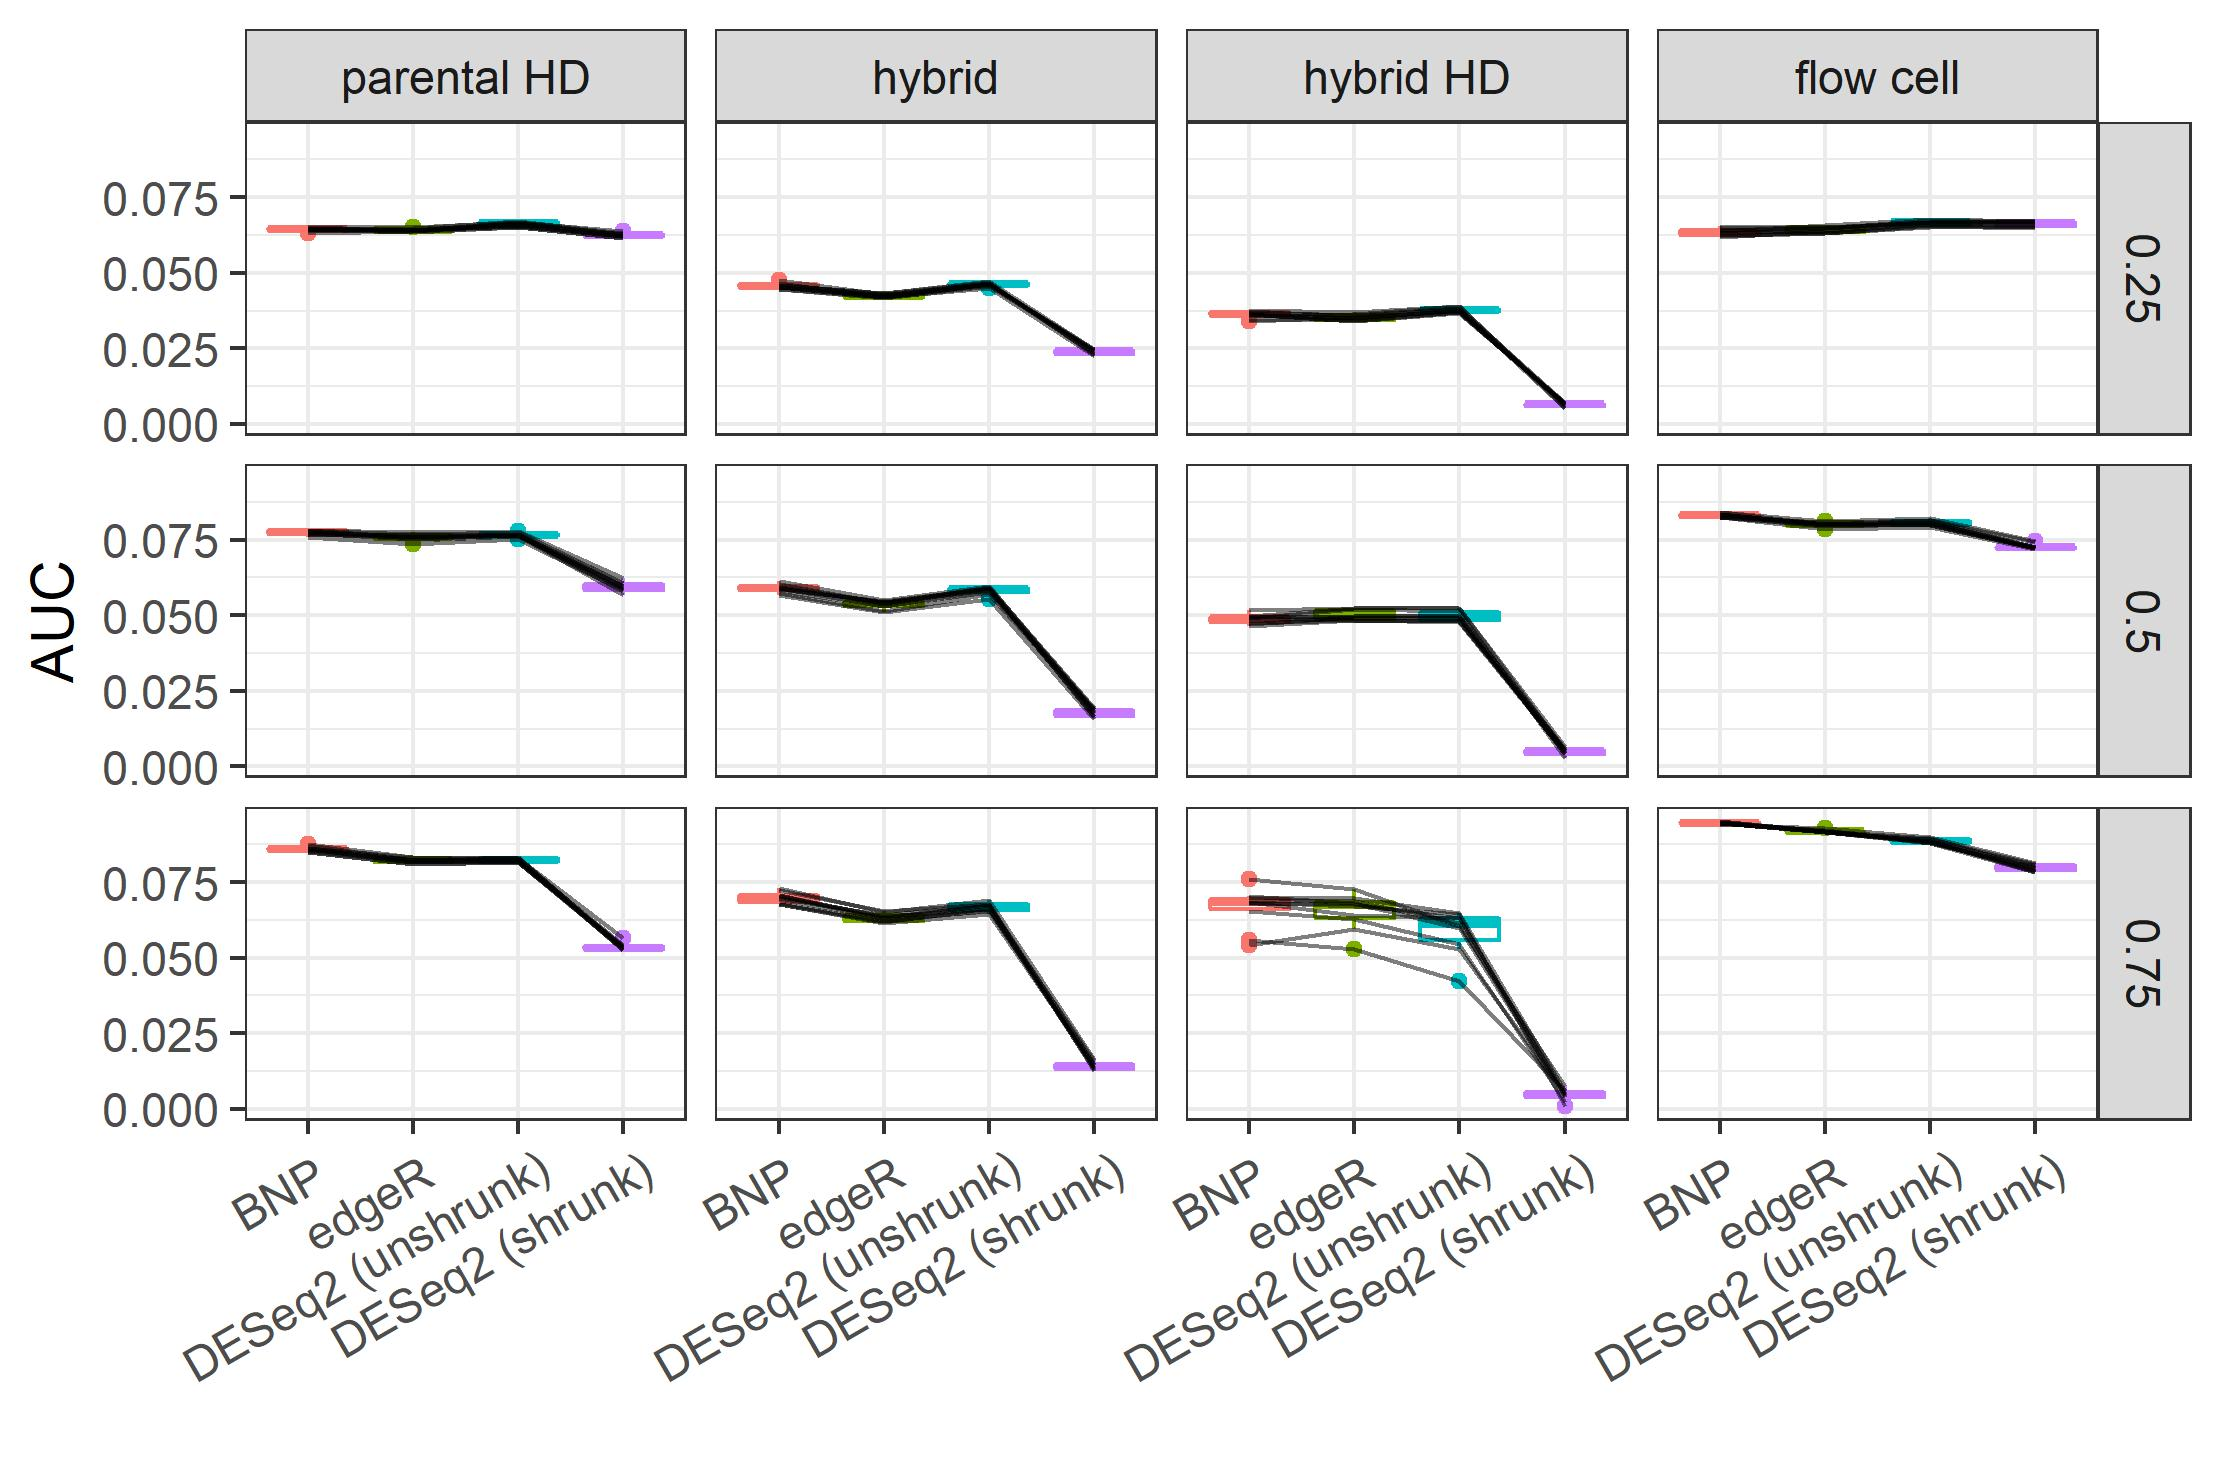
\includegraphics[width=\textwidth]{aud-ss2}
\end{frame}

\begin{frame}[label=current]
  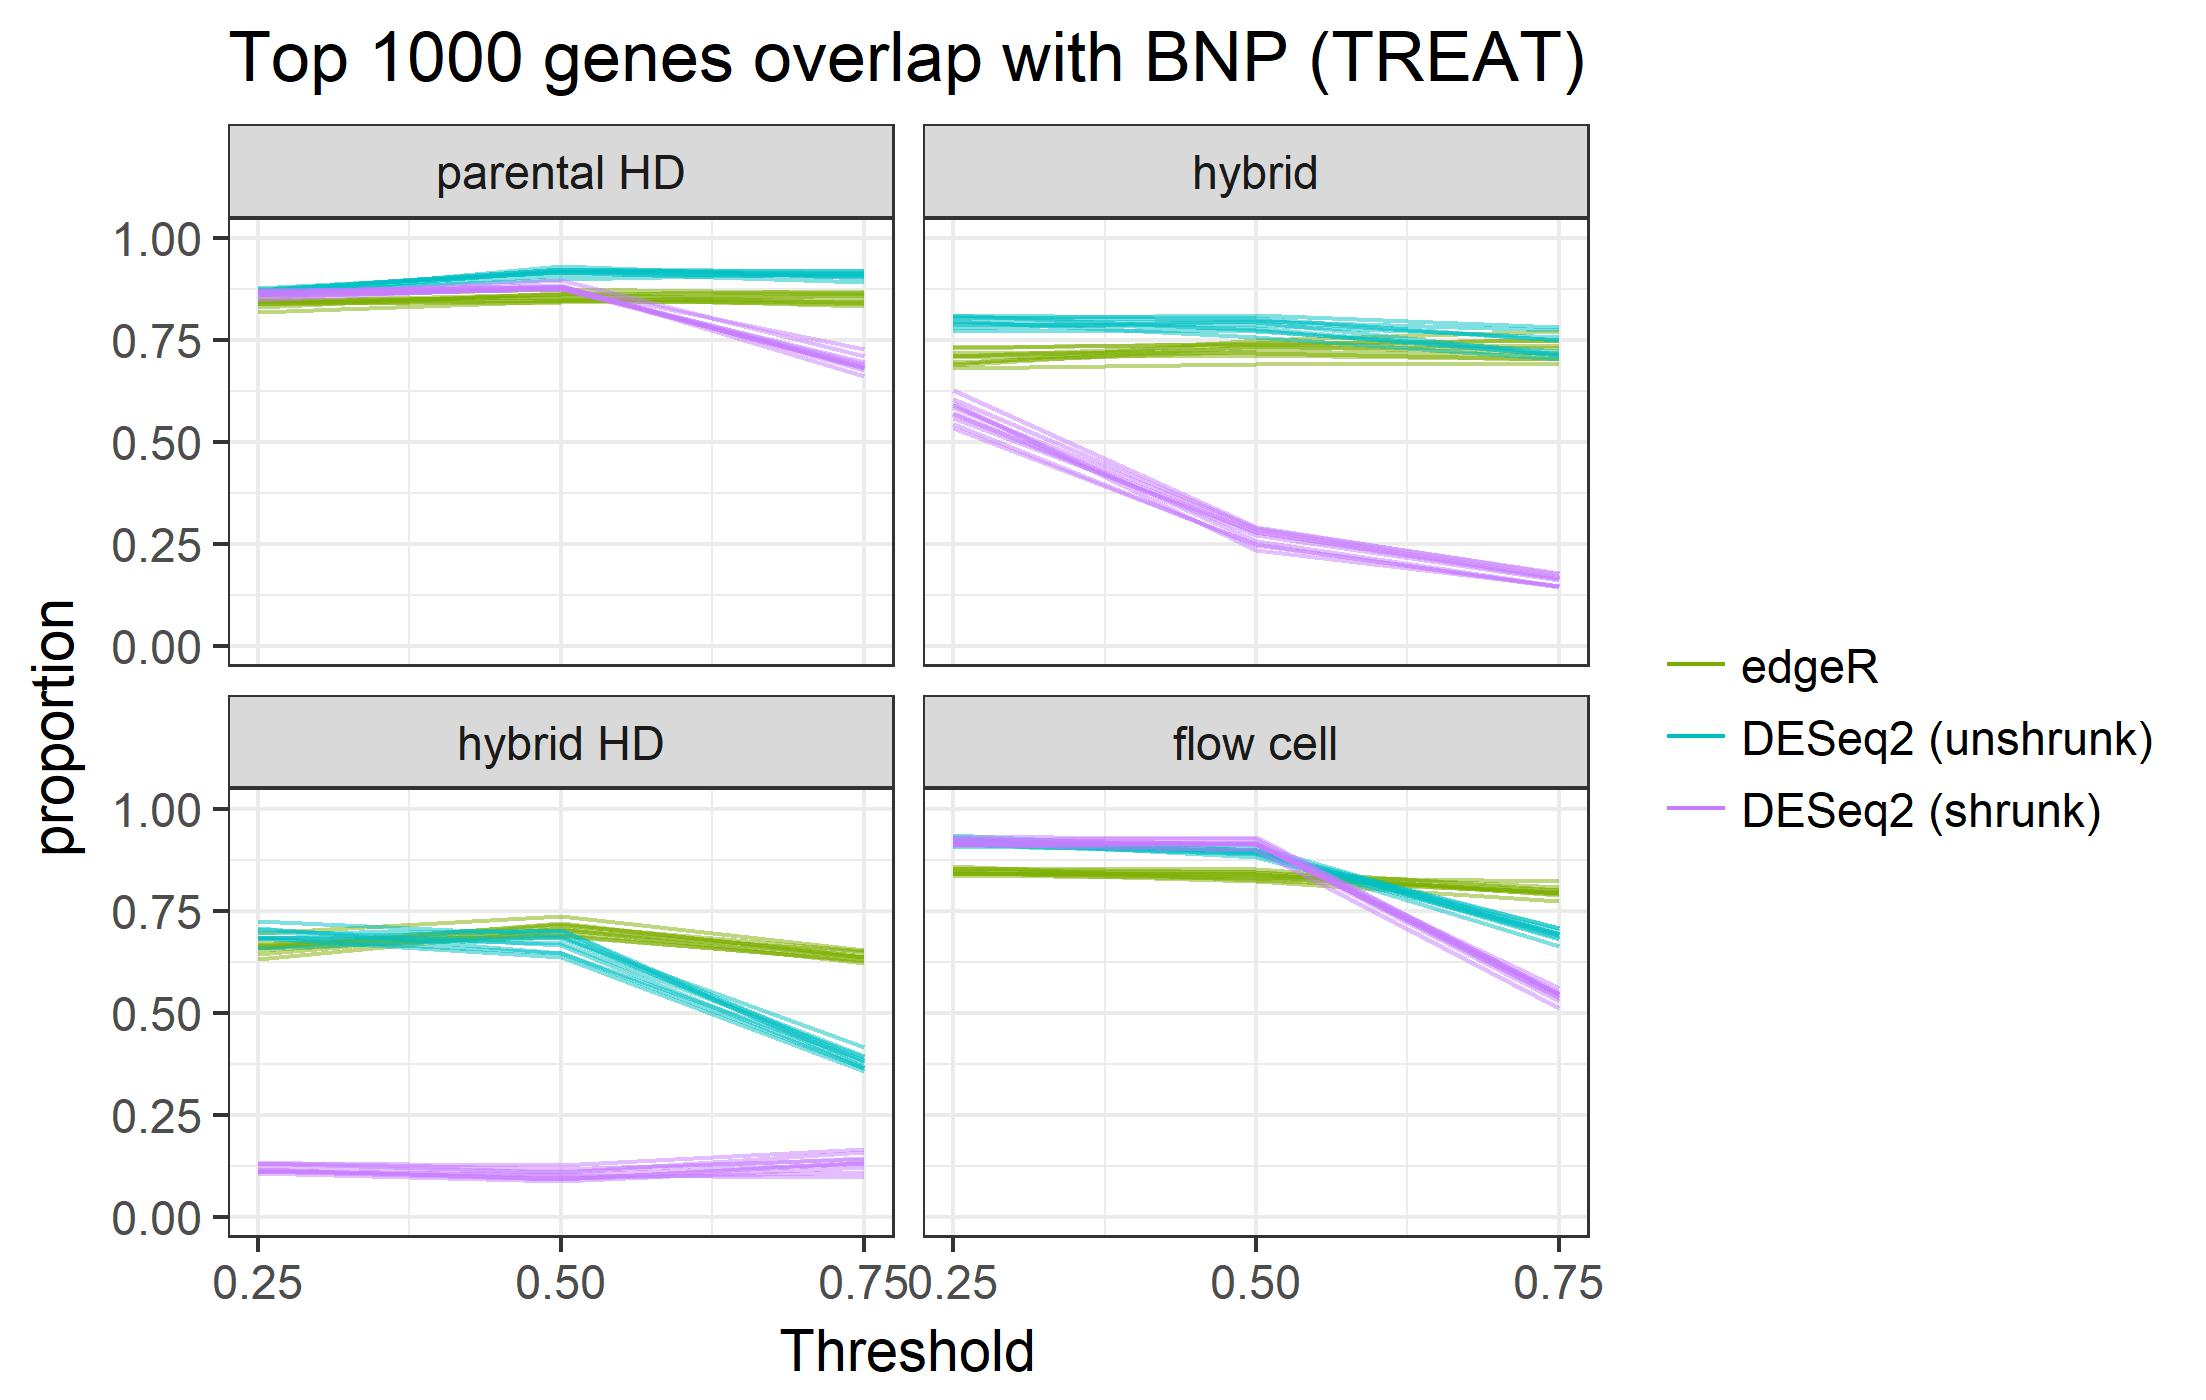
\includegraphics[width=\textwidth]{overlap-ss2-bnp}
\end{frame}

\begin{frame}[label=current]
  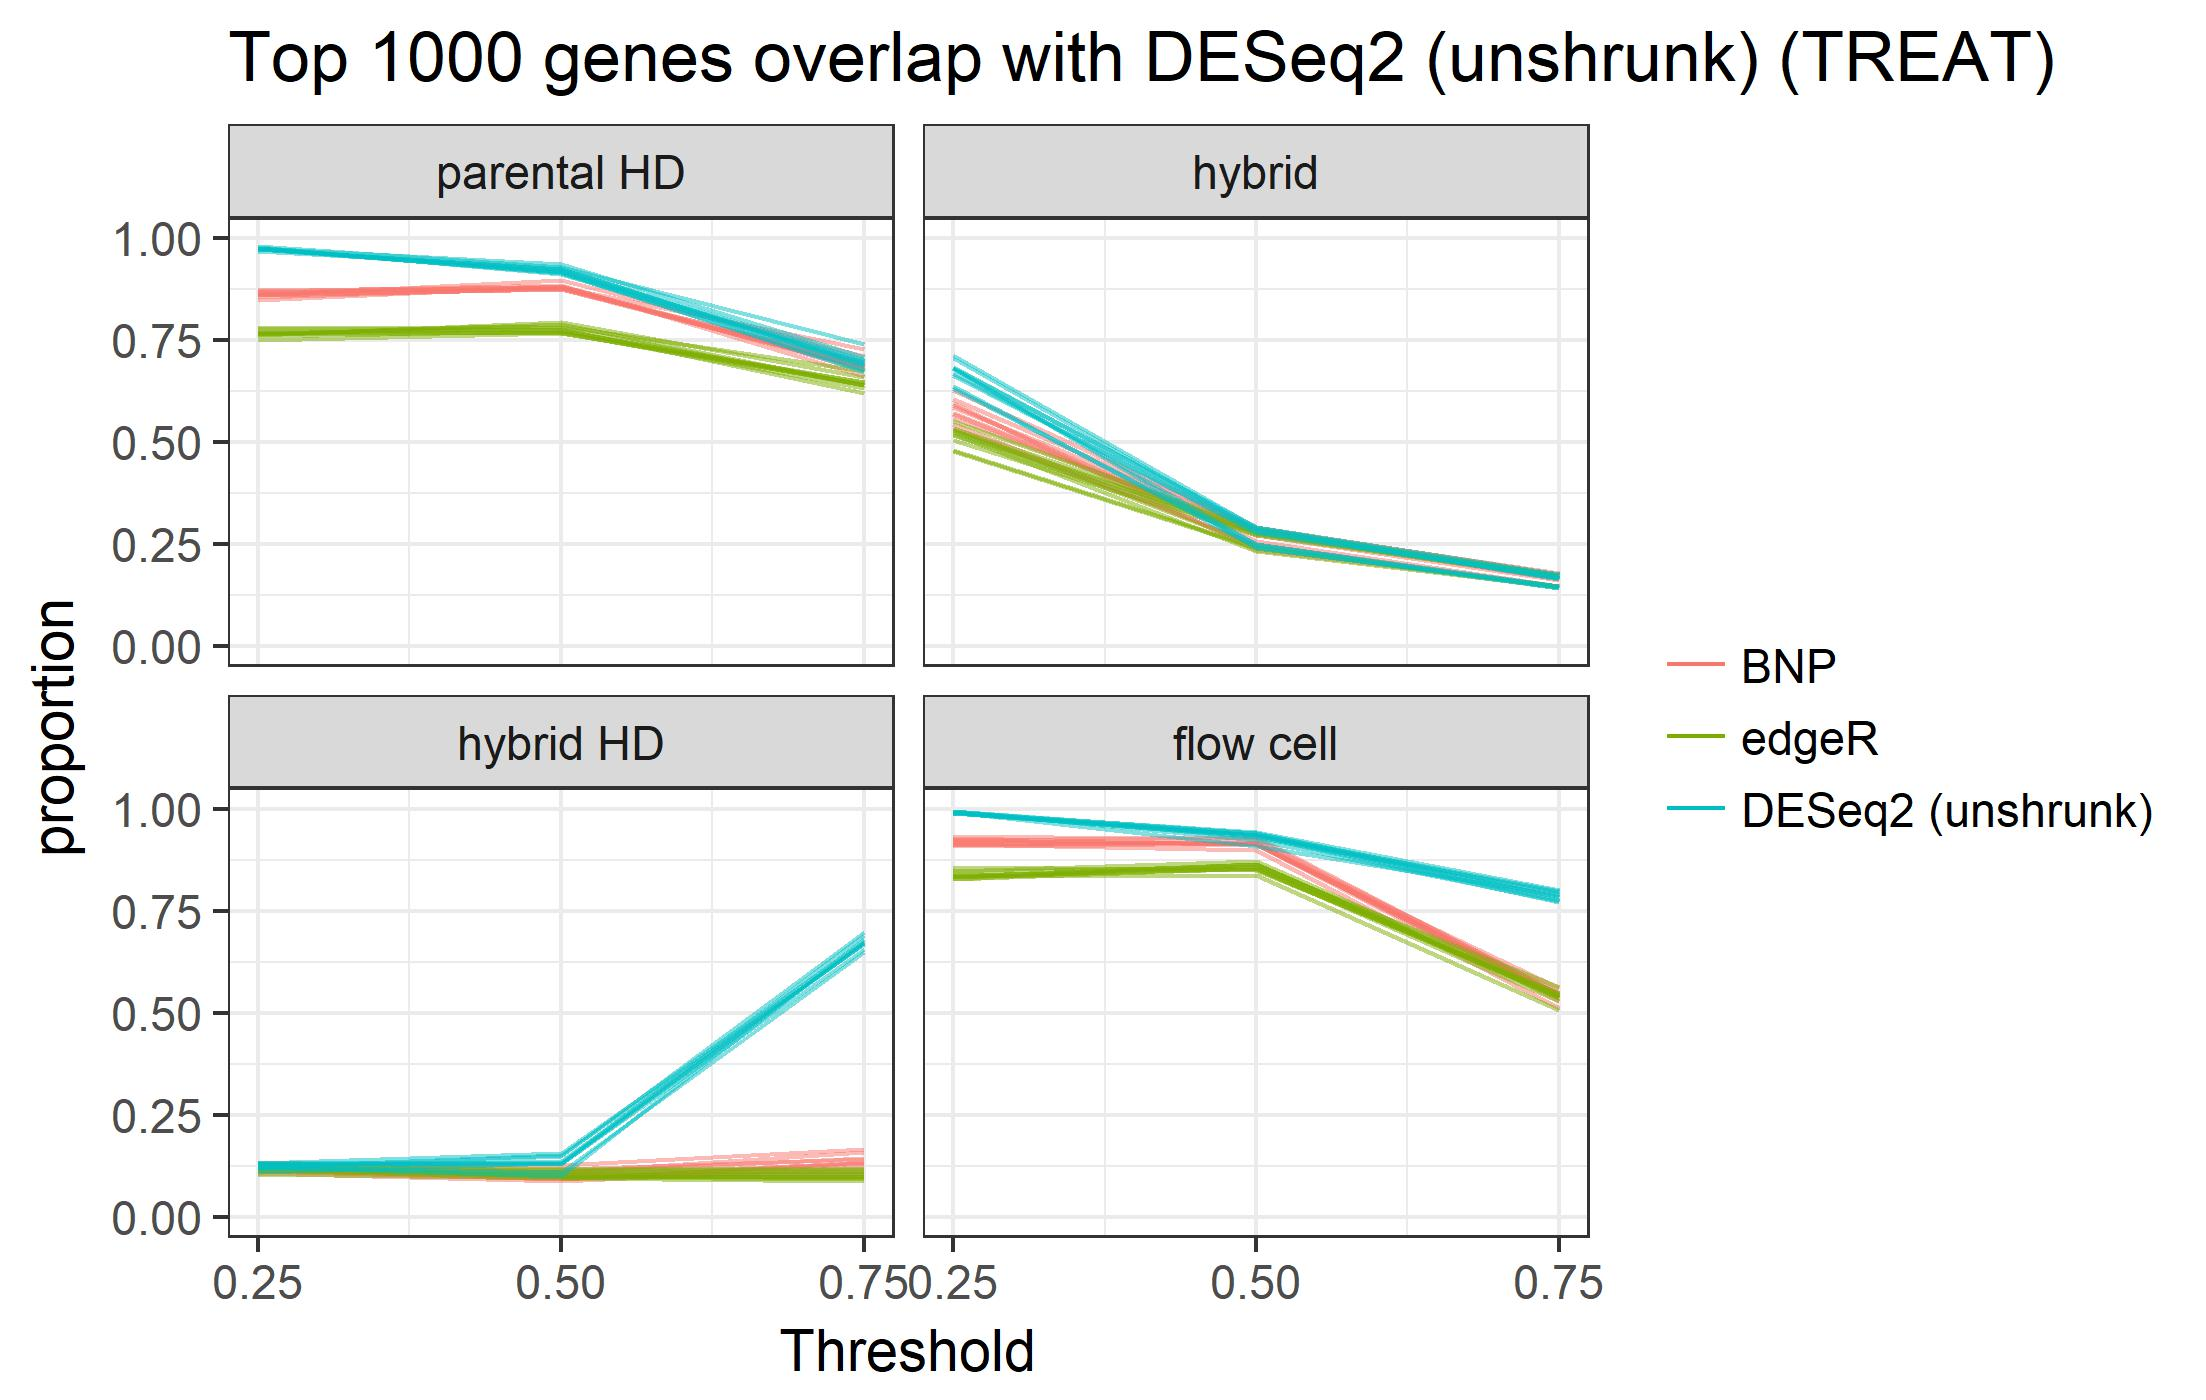
\includegraphics[width=\textwidth]{overlap-ss2-deseq}
\end{frame}

\begin{frame}[label=current]
  \includegraphics[width=.85\textwidth]{ss2-mspe}
\end{frame}

\begin{frame}[label=current]
  \frametitle{Definition of HPH, LPH}
  Recall that:
  {
    \small
    \begin{enumerate}
      \pause \item $H_{HPH,g}: \mbox{hybrid mean expression} > \mbox{high-parent mean expression}$
      \pause \item $H_{LPH,g}: \mbox{hybrid mean expression} < \mbox{low-parent mean expression}$
    \end{enumerate}
  }
    \pause Since there are two hybrids, B73$\times$Mo17 and Mo17$\times$B73, this translates to:
  {
    \small
    \begin{enumerate}
      \item
      \begin{itemize}
        \pause \item$H_{HPH,\mbox{B73\times$Mo17},g}:\; \mbox{hybrid} + \mbox{hybrid HD} > |\mbox{parental HD}|$
        \pause \item$H_{HPH,\mbox{Mo17$\times$B73},g}:\; \mbox{hybrid} - \mbox{hybrid HD} > |\mbox{parental HD}|$
      \end{itemize}
      \item
      \begin{itemize}
        \pause \item$H_{LPH,\mbox{B73$\times$Mo17},g}:\; \mbox{hybrid} + \mbox{hybrid HD} < |\mbox{parental HD}|$
        \pause \item$H_{LPH,\mbox{Mo17$\times$B73},g}:\; \mbox{hybrid} - \mbox{hybrid HD} < |\mbox{parental HD}|$
      \end{itemize}
    \end{enumerate}
  }
\end{frame}

\begin{frame}[label=current]
  \frametitle{Calibration of heterosis probabilities}
  \includegraphics[width=.9\textwidth]{calib-ss2}
\end{frame}

\begin{frame}[label=current]
\frametitle{HPH and LPH probabilities by \citet{paschold} classification}
\includegraphics[width=\textwidth]{orig-compare}
\end{frame}

\begin{frame}[label=current]
  \begin{columns}
      \column{\dimexpr\paperwidth-10pt}
    \frametitle{``Shrinkage" of parameter estimates}
    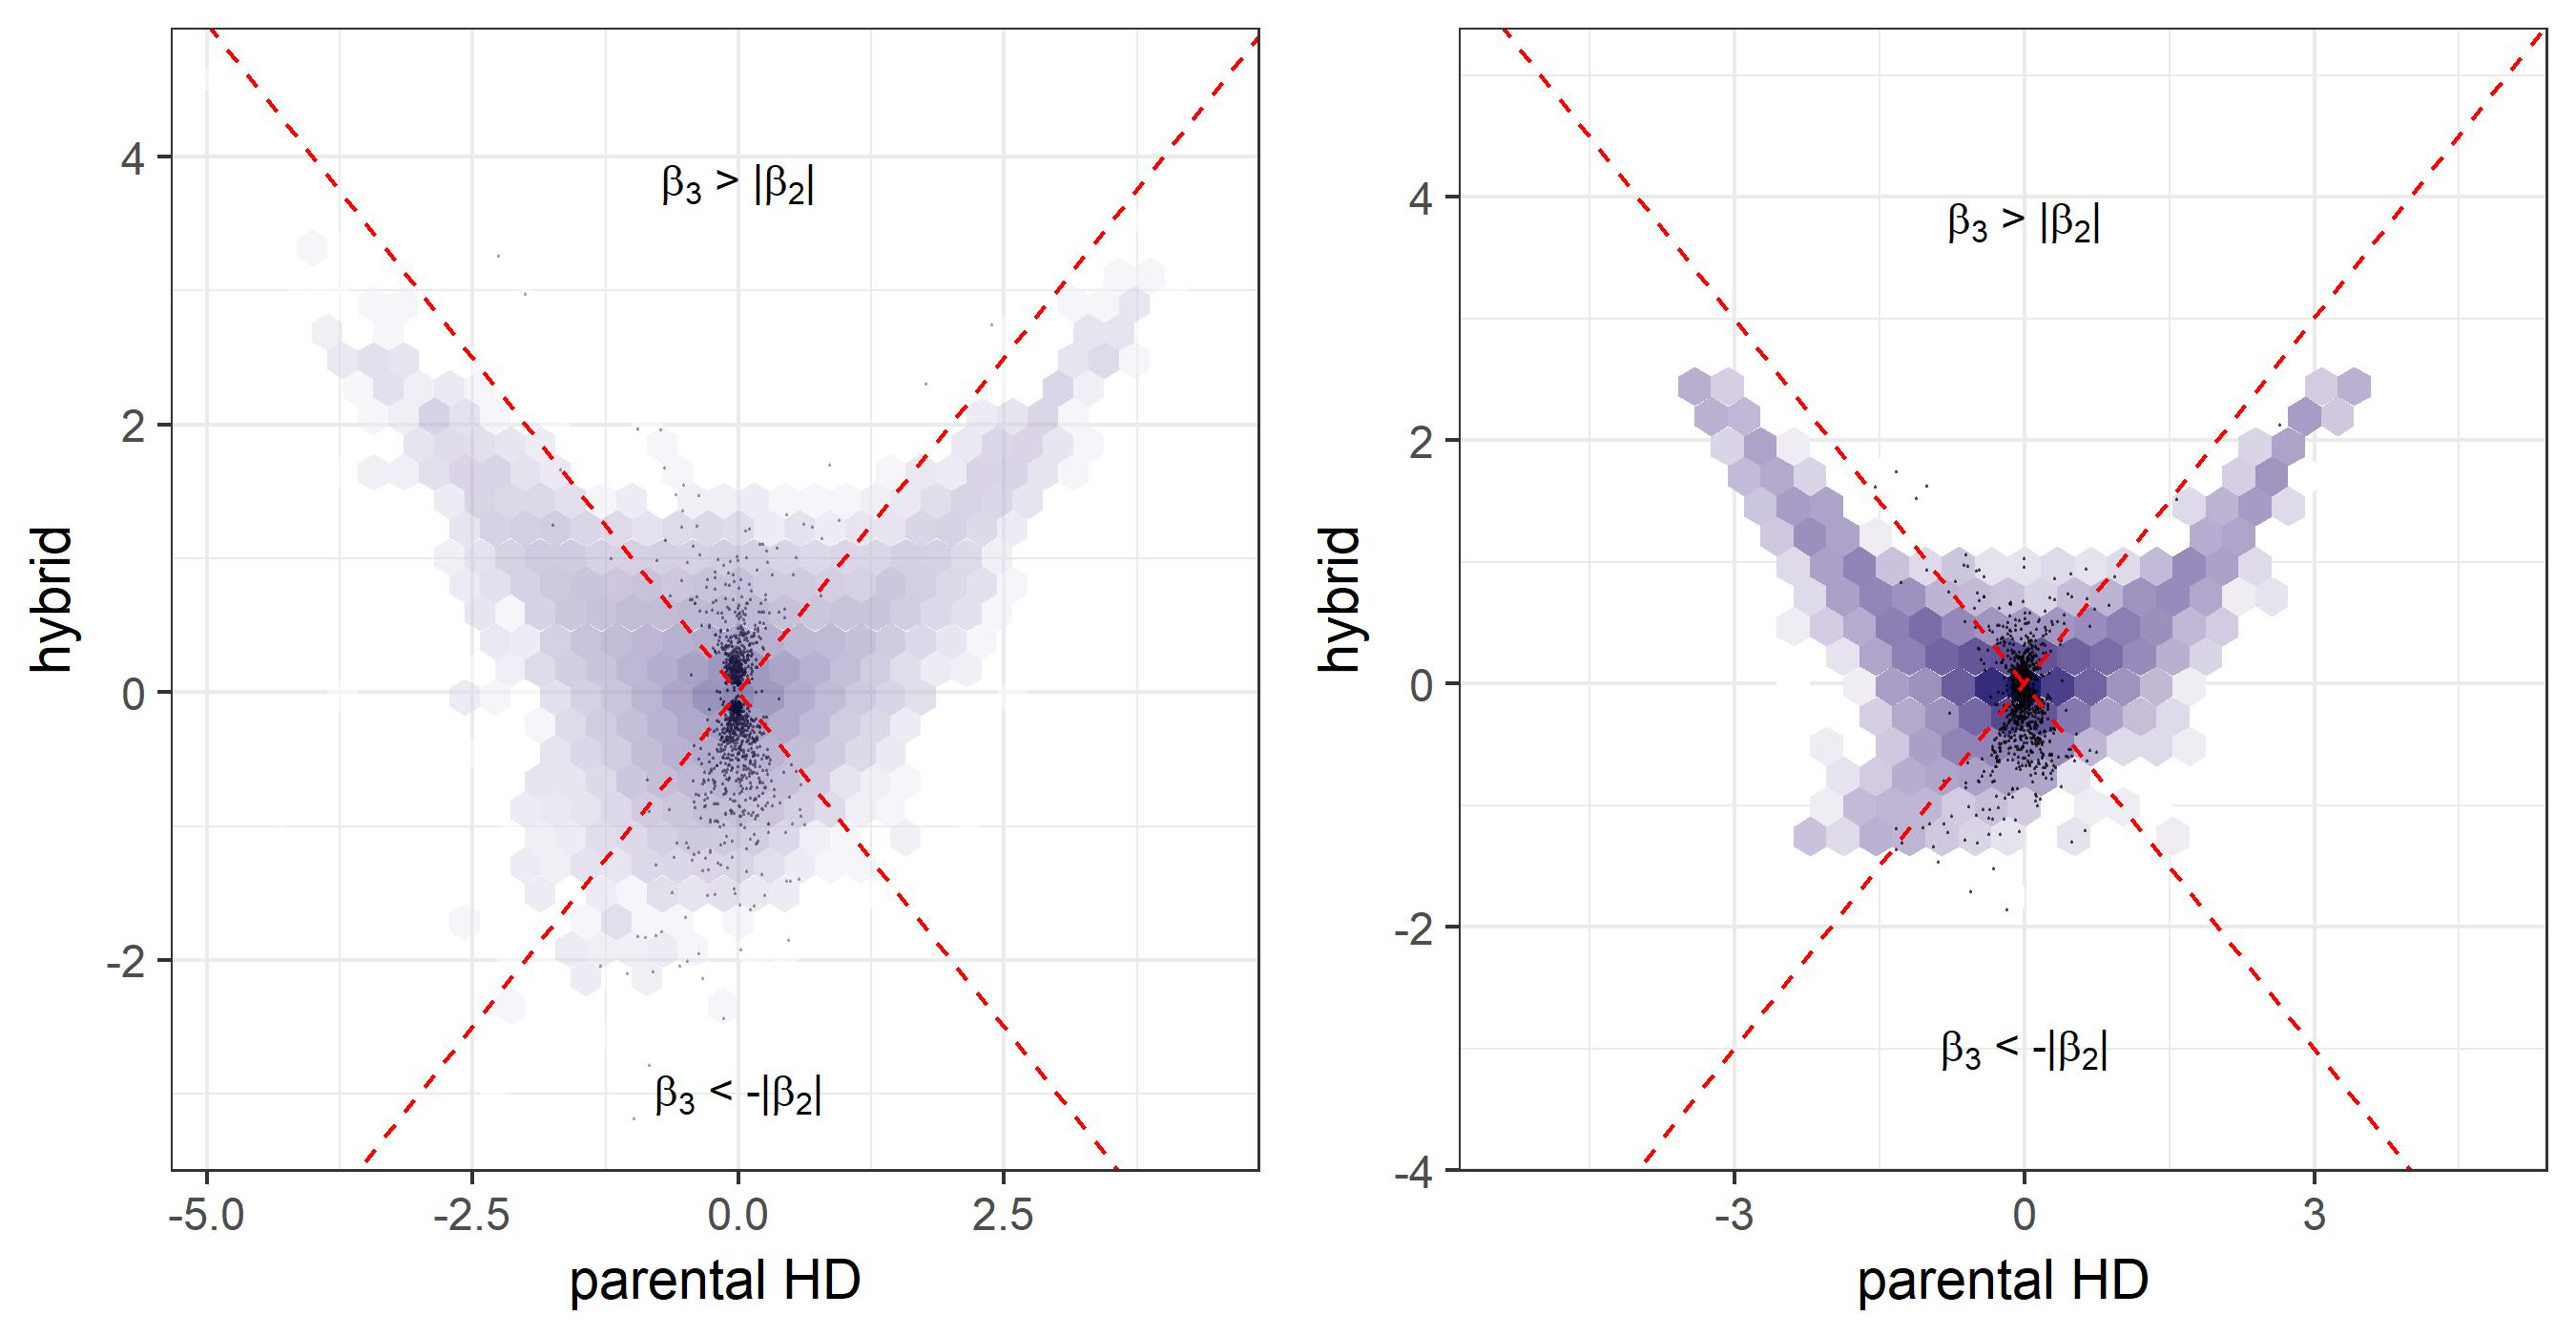
\includegraphics[width=.95\textwidth]{shrinkage}
  \end{columns}
\end{frame}

\begin{frame}[label=current]
  \frametitle{Comparison to results of \citet{landau}}
  Low-parent Heterosis (B73$\times$Mo17)
  \begin{columns}
    \column{\dimexpr\paperwidth-10pt}
    \scalebox{.8}{
      \begin{table}
        \centering
        \begin{tabular}{rrrrrrr|r}
          &  &\multicolumn{6}{c}{Landau and Niemi (2016)}\\
          \toprule
          &  & [0,0.05] & (0.05,0.15] & (0.15,0.85] & (0.85,0.95] & (0.95,1] & total \\
          \midrule
          \multirow{6}{*}{BNP} & [0,0.05]    & 0.283 & 0.083 & 0.116 & 0.001 & 0.000 & 0.483 \\
                               & (0.05,0.15] & 0.017 & 0.037 & 0.129 & 0.003 & 0.001 & 0.186 \\
                               & (0.15,0.85] & 0.009 & 0.025 & 0.254 & 0.017 & 0.009 & 0.313 \\
                               & (0.85,0.95] & 0.000 & 0.000 & 0.007 & 0.002 & 0.002 & 0.011 \\
                               & (0.95,1]    & 0.000 & 0.000 & 0.003 & 0.001 & 0.003 & 0.007 \\
          \midrule
                               & total       & 0.308 & 0.145 & 0.508 & 0.022 & 0.016 & 1.000 \\
          \bottomrule
        \end{tabular}
      \end{table}
    }
  \end{columns}
\end{frame}

\begin{frame}[allowframebreaks]
  \tiny
  \frametitle{References}
  \bibliographystyle{agsm}
  \bibliography{../mybib}
\end{frame}

\begin{frame}%[label=current]
  \frametitle{Acknowledgment}
  \small%
  This research was supported by National Institute of General Medical Sciences (NIGMS) of the National Institutes of Health and the joint National Science Foundation / NIGMS Mathematical Biology Program under award number R01GM109458. The content is solely the responsibility of the authors and does not necessarily represent the official views of the National Institutes of Health or the National Science Foundation.
\end{frame}

\end{document}